\documentclass{ieeeaccess}
\usepackage{cite}
\usepackage{amsmath,amssymb,amsfonts}
\usepackage{graphicx}
\usepackage{textcomp}
\usepackage{booktabs}
\usepackage{array}
\usepackage{bm}
\sloppy

\makeatletter
\AtBeginDocument{\DeclareMathVersion{bold}
\SetSymbolFont{operators}{bold}{T1}{times}{b}{n}
\SetSymbolFont{NewLetters}{bold}{T1}{times}{b}{it}
\SetMathAlphabet{\mathrm}{bold}{T1}{times}{b}{n}
\SetMathAlphabet{\mathit}{bold}{T1}{times}{b}{it}
\SetMathAlphabet{\mathbf}{bold}{T1}{times}{b}{n}
\SetMathAlphabet{\mathtt}{bold}{OT1}{pcr}{b}{n}
\SetSymbolFont{symbols}{bold}{OMS}{cmsy}{b}{n}
\renewcommand\boldmath{\@nomath\boldmath\mathversion{bold}}}
\makeatother

\usepackage[colorlinks=true,linkcolor=accessblue,citecolor=accessblue,urlcolor=accessblue,bookmarks=true]{hyperref}

\def\BibTeX{{\rm B\kern-.05em{\sc i\kern-.025em b}\kern-.08em
    T\kern-.1667em\lower.7ex\hbox{E}\kern-.125emX}}

\begin{document}
\history{Manuscript prepared for IEEE Access submission.}
\doi{Pending}

\title{TRUEGUARD: An Empirical Study of White-Box Hallucination Detection, Domain Shift, and Selective Prediction in Large Language Models}

\author{\uppercase{Yogesh Ravi M}\authorrefmark{1} AND
\uppercase{T. S. Pradeep Kumar}\authorrefmark{1}, \IEEEmembership{Senior Member, IEEE}}

\address[1]{School of Computer Science and Engineering, Vellore Institute of Technology, Chennai, Tamil Nadu, India (e-mail: yogeshravi4343@gmail.com; tspradeepkumar@vit.ac.in)}

\markboth
{Y.\ Ravi M and T.\ S.\ Pradeep Kumar: TRUEGUARD: White-Box Hallucination Detection, Domain Shift, and Selective Prediction}
{Y.\ Ravi M and T.\ S.\ Pradeep Kumar: TRUEGUARD: White-Box Hallucination Detection, Domain Shift, and Selective Prediction}

\corresp{Corresponding author: T. S. Pradeep Kumar (e-mail: tspradeepkumar@vit.ac.in).}

\begin{abstract}
Large language models (LLMs) frequently produce fluent text that is factually incorrect or unsupported by context. Established black-box hallucination detectors sample multiple responses and score consistency with an external natural language inference (NLI) model, increasing decoding cost and requiring an auxiliary classifier. White-box detectors estimate hallucination risk in one forward pass from internal activations, attention weights, and token probabilities, yet their reliability under dataset artifacts, cross-domain shift, and closed-book selective prediction remains incompletely understood on small frozen models. This paper presents an empirical study of TRUEGUARD, a single-pass white-box framework instrumented on frozen TinyLlama-1.1B-Chat-v1.0 without updating base weights. TRUEGUARD extracts four internal signals, namely Internal State Probe (ISP), Attention Anomaly Score (AAS), Energy/Entropy Monitor (EEM), and Directional Semantic Trajectory (DST), fused by logistic regression and paired with a three-tier response controller. Across ten datasets (32,590 sequences), three findings emerge. First, raw HaluEval AUROCs (0.9880 QA, 0.9936 Summarization) are heavily inflated by length (0.9572 on QA) and answer-text TF-IDF (0.9661 QA, 0.9539 Summarization); yet TRUEGUARD significantly beats TF-IDF under strict length matching ($|\Delta L| \le 2$; 0.7901 to 0.9939 AUROC, $p \le 0.035$), with ISP carrying over 96\% of fusion weight. Second, zero-shot pooled probes collapse to chance on four unseen benchmarks (0.4597 to 0.5205), consistent with higher within-domain (+0.1125 to +0.6707 at $N=900$) than cross-domain (-0.0151 to +0.0204) probe alignment, while target-only few-shot refitting ($K=250$) yields task-dependent gains on FaithDial (0.8231), FEVER (0.7325), and WikiBio (0.6698) but ties 1D length on XSum (0.6456 vs.\ 0.6445) and trails simple baselines at $K=50$. Third, on 250 closed-book TriviaQA generations, target-refitted TRUEGUARD ($K=250$; 0.7876 AUROC, 0.4360 AURC) significantly outperforms label-free 10-sample Semantic Entropy (0.6859), Predictive Entropy (0.6583), and NLL (0.4678), and matches label-free SelfCheckGPT-NLI (0.7477, $p_{\text{Holm}}=0.478$), whereas zero-shot pooled TRUEGUARD scores 0.5504. At 46.0\% coverage, pure selective abstention achieves 55.65\% accuracy (64/115) versus 54.78\% (63/115) for the full three-tier controller, showing no measurable benefit from active resampling or retrieval.
\end{abstract}

\begin{keywords}
Abstention, dataset artifacts, domain shift, few-shot refitting, hallucination detection, internal representations, large language models, selective prediction, white-box probing.
\end{keywords}

\titlepgskip=-21pt

\maketitle

% ==============================================================================
\section{Introduction}
\label{sec:introduction}

\subsection{Background and Motivation}
\PARstart{L}{arge} language models (LLMs) are now used across question answering, summarization, dialogue, and decision support. Even when their writing appears clear and well structured, these models regularly produce hallucinations, meaning outputs that contradict factual knowledge, invent unsupported details, or depart from the provided source text \cite{review35,review18}. Because fabricated answers often resemble correct ones in tone and grammar, users cannot easily tell when a response is reliable. That uncertainty directly weakens human trust in language model outputs \cite{review19,review03}.

Detecting incorrect answers at inference time is particularly difficult when applications rely on small, frozen open-weight models for privacy, memory, or latency reasons. Several established black-box detectors, including SelfCheckGPT \cite{review21} and Semantic Entropy \cite{kuhn2023semantic,farquhar2024detecting}, sample multiple stochastic responses for each prompt and compare them using an external natural language inference (NLI) model. Although black-box methods require no access to internal model weights, generating many responses per query increases computational work and requires serving a second neural model. White-box methods offer a single-pass alternative. By inspecting hidden activations, attention weights, and token probability distributions during one forward pass, a lightweight classifier can estimate hallucination risk without modifying the frozen language model or generating extra candidate answers \cite{review27,review01,review12}.

\subsection{Problem Statement}
Despite encouraging in-domain results reported in the white-box probing literature, three practical issues complicate real-world use. First, standard hallucination benchmarks such as HaluEval \cite{review29} pair human or reference answers with synthetically generated hallucinations. High accuracy on those benchmarks may reflect differences in answer length or writing style rather than genuine detection of factual errors. Second, supervised probes trained on one group of benchmarks often lose accuracy when applied to a new domain. Practitioners therefore need to know whether small amounts of target-domain labeled data can restore performance, and whether refitted white-box probes actually outperform simpler one-dimensional or text-only baselines. Third, when a detector is connected to a response controller that can resample, retrieve external evidence, or abstain, evaluation must separate the accuracy gained by abstaining on risky questions from the net effect of active correction attempts.

\subsection{Research Gap}
Previous studies have investigated linear hidden-state probing \cite{review27,review28}, attention patterns \cite{review09,review11}, token entropy and energy \cite{review04,review17}, multi-sample black-box consistency \cite{review21}, and retrieval-based revision \cite{review25,review33}. However, these components are usually studied in separate experimental setups, on different models, or without joint artifact and baseline controls. Little empirical evidence examines all four internal signal families inside one frozen small language model across ten datasets while simultaneously quantifying length and TF-IDF benchmark artifacts, comparing within-domain and cross-domain probe directions at equal sample sizes, benchmarking target-only few-shot refitting against simple baselines, and auditing abstention versus active multi-tier intervention alongside reproduced external baselines on the same held-out closed-book generations.

\subsection{Research Objectives and Questions}
This study evaluates TRUEGUARD on frozen \texttt{TinyLlama/TinyLlama-1.1B-Chat-v1.0} to answer four focused research questions. The first question asks how accurately single-pass white-box signals detect hallucinations in-domain and how much performance remains after controlling for answer length and surface-text TF-IDF artifacts. The second question asks why pooled white-box probes fail under zero-shot domain shift and what within-domain versus cross-domain probe alignment and length-controlled entropy checks reveal about that failure. The third question asks when target-domain few-shot refitting, trained from scratch on 50, 100, or 250 target examples, outperforms source-risk recalibration and simple one-dimensional or text-only baselines. The fourth question asks how target-refitted single-pass white-box detection compares with label-free multi-sample external baselines (SelfCheckGPT-NLI and Semantic Entropy) on closed-book TriviaQA generations, and whether a three-tier active controller provides any net benefit over pure selective abstention at matched coverage.

\subsection{Main Research Contributions}
Rather than presenting individual white-box signals or selective routing as new algorithmic inventions, this work uses TRUEGUARD as a unified experimental framework for a controlled empirical study. The manuscript makes three main evidence-backed empirical contributions supported by an auditable single-pass instrumentation pipeline.

First, across five in-domain benchmarks (18,141 rows), we show that headline HaluEval AUROC values (0.9880 on HaluEval-QA and 0.9936 on HaluEval-Summarization) are heavily influenced by answer-length and surface-style artifacts, with length alone reaching 0.9572 on HaluEval-QA and answer-text TF-IDF alone reaching 0.9661 and 0.9539 on those two datasets. Even after strict length matching within two tokens, however, TRUEGUARD significantly outperforms answer-text TF-IDF on all four paired benchmarks (gains of +0.0331 to +0.0829 AUROC, $p \le 0.035$), while ablation experiments show that ISP carries more than 96\% of the fusion weight and that four-sensor fusion does not consistently outperform ISP alone.

Second, across four initially unseen benchmarks (13,949 rows), we document zero-shot collapse of pooled white-box probes (0.4597 to 0.5205 AUROC) and failure of source-risk recalibration (0.4957 to 0.5242). Equal-sample-size diagnostics ($N = 900$) show substantially higher within-domain split-half probe weight alignment (+0.1125 to +0.6707) than cross-domain alignment (-0.0151 to +0.0204), and length-controlled entropy checks distinguish genuine length-free EEM signal on FaithDial (0.7662) and XSum (0.6648) from length-confounded inversion on HaluEval-QA. Target-domain few-shot refitting with zero source weight transfer reveals a clear sample-efficiency boundary: simpler baselines outperform TRUEGUARD at $K = 50$, whereas $K = 250$ refitting (under 2~s on CPU) yields task-dependent gains on FaithDial (0.8231), FEVER (0.7325), and WikiBio (0.6698), while matching 1D length on XSum (0.6456 vs.\ 0.6445).

Third, on 250 held-out closed-book TriviaQA generations, we show that target-refitted single-pass TRUEGUARD ($K = 250$ calibration examples, 0.7876 AUROC, 0.4360 AURC) significantly outperforms label-free 10-sample Semantic Entropy (0.6859, $p_{\text{Holm}} = 0.012$), Predictive Entropy (0.6583, $p_{\text{Holm}} = 0.006$), and verified length-normalized NLL (0.4678, $p_{\text{Holm}} = 0.006$), and performs competitively with label-free 10-sample SelfCheckGPT-NLI (0.7477, $p_{\text{Holm}} = 0.478$, not statistically significant) without extra generations or an external NLI model. In contrast, zero-shot pooled TRUEGUARD obtains only 0.5504 AUROC. Finally, a forensic mitigation audit at 46.0\% coverage establishes that pure selective abstention (64/115 correct, 55.65\%) drives the error reduction, while the full three-tier controller (63/115 correct, 54.78\%; four errors repaired and three correct answers broken) shows no measurable net benefit from active regeneration or Wikipedia retrieval on this 1.1B model.

\subsection{Organization of the Paper}
Section~\ref{sec:related} reviews related research on hallucinations, white-box and black-box detection, domain shift, benchmark artifacts, and mitigation. Section~\ref{sec:framework} describes the TRUEGUARD framework, the frozen TinyLlama model, the four sensor formulations, the fusion classifier, and the response controller. Section~\ref{sec:methodology} details the datasets, feature extraction, artifact controls, target-domain refitting protocol, external baselines, and statistical tests. Section~\ref{sec:results} reports the experimental results. Section~\ref{sec:discussion} interprets the findings, practical trade-offs, and limitations. Section~\ref{sec:conclusion} summarizes the conclusions and directions for future work.

% ==============================================================================
\section{Related Work}
\label{sec:related}

\subsection{Hallucinations in Large Language Models}
Surveys of natural language generation commonly divide hallucinations into intrinsic errors, which contradict the provided source text, and extrinsic errors, which introduce claims that cannot be verified from the source \cite{review35,review18}. Empirical evaluations of instruction-tuned models demonstrate that factual errors remain frequent across closed-book question answering, long-form biography generation, and open-domain dialogue \cite{review37,review23}. Standardized benchmarks such as TruthfulQA \cite{review22}, HaluEval \cite{review29}, and self-contradiction test suites \cite{review36} have enabled structured comparison of detection methods, while broader trustworthiness studies examine how unreliable outputs affect user calibration and trust \cite{review03,review19}.

\subsection{Internal-State Hallucination Detection}
Internal-state detectors examine whether a frozen model's hidden activations separate truthful statements from fabricated ones. Azaria and Mitchell \cite{review27} proposed SAPLMA, which trains lightweight classifiers on intermediate hidden layers to predict statement truthfulness. Later studies extended internal representation monitoring in several directions, including unsupervised real-time hidden-state tracking in MIND \cite{review01}, prompt-guided representation probing in PRISM \cite{review02}, deeper layer-wise representation analysis \cite{review05}, and representation-shift monitoring in HalluShift \cite{review13}. Other work trains linear probes over hidden states to approximate semantic entropy in a single pass \cite{review14}, or shifts activations along truthful directions during decoding, as in Inference-Time Intervention (ITI) \cite{review28} and Truth Forest \cite{review38}. Across these studies, hidden-state probing achieves strong in-domain discrimination, though its sensitivity to dataset construction and domain shift remains an active concern.

\subsection{Attention-Based and Uncertainty-Based Detection}
A second body of research focuses on self-attention distributions and output token uncertainty. LLM-Check \cite{review12} evaluates hidden-state eigenvalues, attention maps, and token perplexity across hallucination tasks. More recent studies trace intrinsic and extrinsic hallucinations through attention patterns \cite{review09} and identify uncertainty-aware attention heads for unsupervised scoring \cite{review11}. On the logit side, uncertainty quantification surveys \cite{review07} review predictive entropy, token-level entropy production rates \cite{review17}, and energy-based scores that extend standard Shannon entropy \cite{review04}. In black-box settings where internal weights are unavailable, SelfCheckGPT \cite{review21} generates multiple stochastic samples and measures contradiction using NLI or text overlap. Semantic Entropy \cite{kuhn2023semantic,farquhar2024detecting} similarly draws multiple responses, clusters semantically equivalent answers using bidirectional NLI entailment, and computes entropy over the resulting semantic clusters.

\subsection{Cross-Domain Generalization and Benchmark Artifacts}
High detection scores on one benchmark do not automatically imply generalizable factual verification. Synthetic benchmarks such as HaluEval \cite{review29} construct negative examples by prompting an LLM to modify or fabricate answers, which can create systematic differences in answer length, vocabulary, or phrasing relative to reference answers. Supervised probes trained on high-dimensional activations can easily exploit those surface cues. In addition, token-level uncertainty metrics may exhibit opposite associations on teacher-forced synthetic pairs versus naturally generated model errors. Evaluating white-box detectors without length controls, text-only TF-IDF baselines, and strict cross-domain splits therefore risks overestimating real-world reliability.

\subsection{Hallucination Mitigation and Selective Prediction}
When a potential error is detected, systems either attempt active correction or refuse to answer. Active approaches include retrieval-augmented generation (RAG) \cite{review25}, self-reflective retrieval in Self-RAG \cite{review26}, structured self-verification in Chain-of-Verification (CoVe) \cite{review24}, tool-based post-hoc revision in RARR \cite{review33}, FacTool \cite{review34}, and CRITIC \cite{review39}, multi-agent debate \cite{review31}, and behaviorally calibrated reinforcement learning \cite{review15}. When external verification is weak or a small model lacks the underlying factual knowledge, selective prediction provides a conservative alternative. By abstaining on high-risk inputs and evaluating selective accuracy across coverage levels using the area under the risk-coverage curve (AURC) \cite{geifman2017selective}, a system can trade coverage for lower error rates without relying on uncertain self-repair.

\subsection{Positioning of TRUEGUARD}
TRUEGUARD integrates four established internal signal families (ISP, AAS, EEM, DST) into a single frozen-model pipeline and uses that pipeline to perform a controlled empirical evaluation. Rather than proposing a single sensor as a universal solution, this study evaluates how much in-domain accuracy survives length and TF-IDF controls, diagnoses zero-shot domain-shift failure using equal-sample-size representation checks, maps when target-only few-shot refitting beats simple baselines, compares target-refitted single-pass detection against label-free multi-sample SelfCheckGPT-NLI and Semantic Entropy with explicit supervision disclosure, and tests whether a three-tier active controller improves upon pure selective abstention on a small frozen model.

% ==============================================================================
\section{Proposed TRUEGUARD Framework}
\label{sec:framework}

\begin{figure*}[t]
\centering
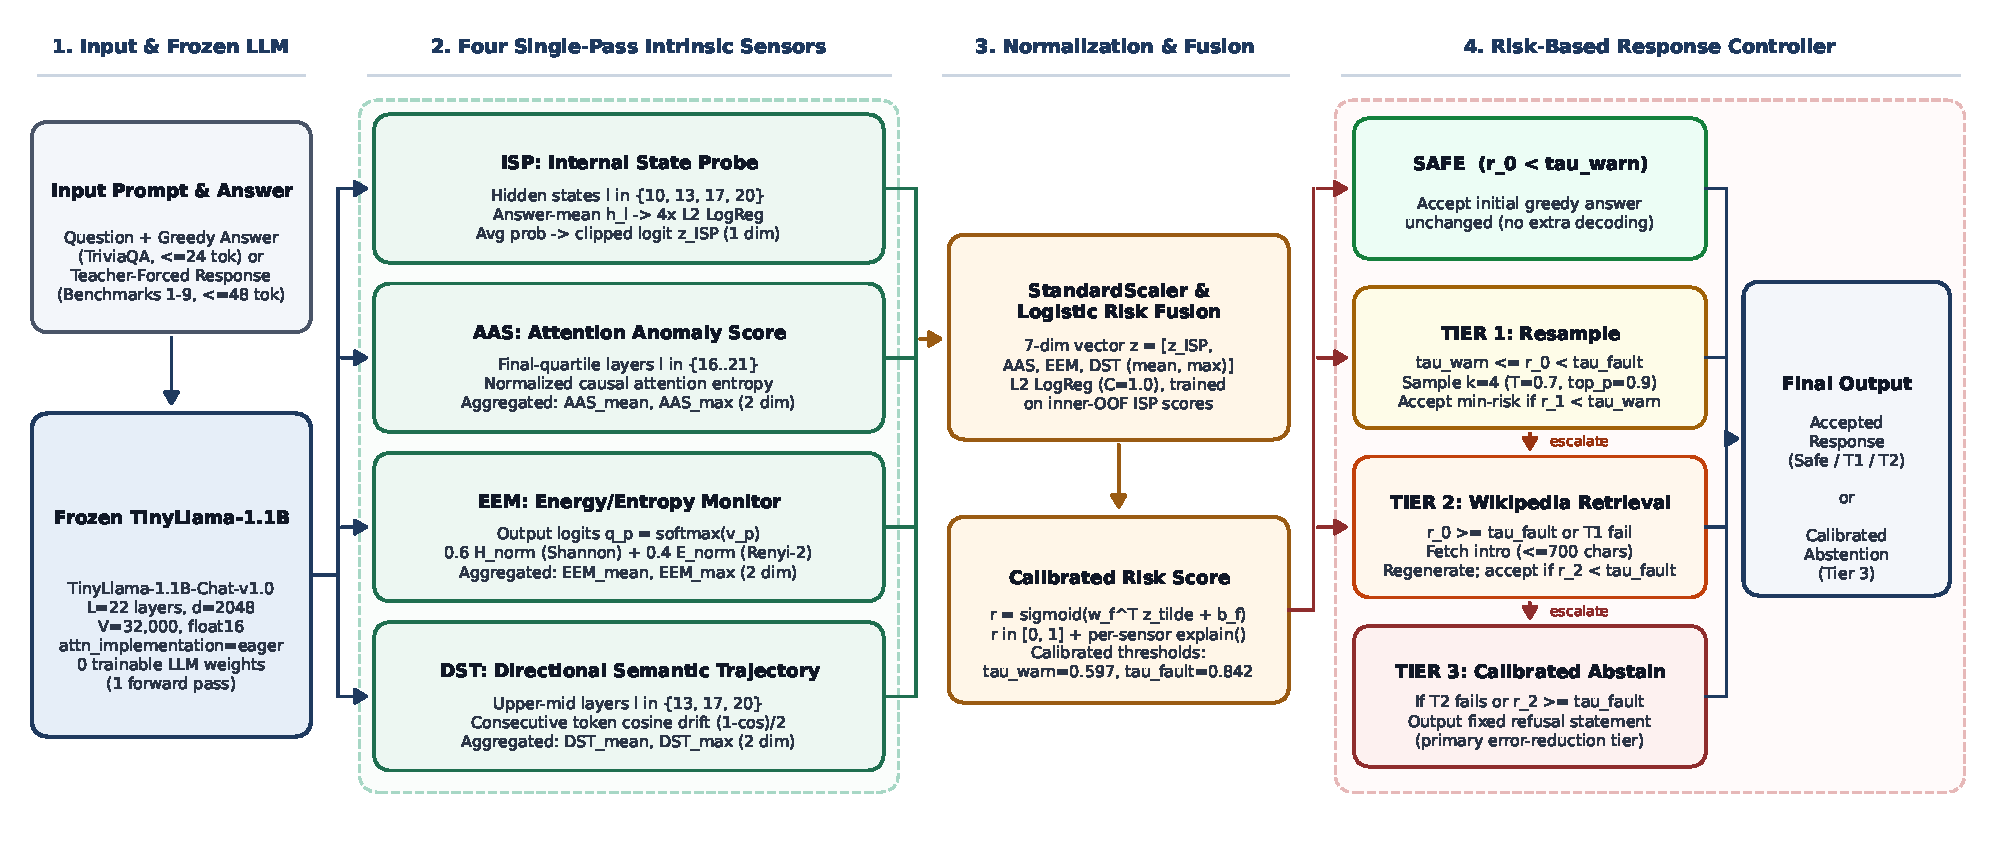
\includegraphics[width=\textwidth]{figures/Fig1_TRUEGUARD_Architecture.pdf}
\caption{Overview of the TRUEGUARD single-pass white-box framework attached to frozen TinyLlama-1.1B-Chat-v1.0. Four intrinsic signal families (ISP, AAS, EEM, DST) are extracted in parallel from intermediate hidden states, final-quartile causal attention weights, and output logits in one forward pass, normalized and fused by an L2-regularized logistic classifier into a calibrated hallucination risk score $r \in [0, 1]$, and routed through a three-tier selective response controller (SAFE, TIER 1 Resample, TIER 2 Wikipedia Retrieval, TIER 3 Calibrated Abstain). Conceptual architecture diagram matching the implemented \texttt{tg\_pipeline.py} and \texttt{tg\_controller.py} modules.}
\label{fig:arch}
\end{figure*}

\subsection{System Architecture}
TRUEGUARD is a white-box risk-monitoring and selective-response framework attached to a frozen autoregressive language model. No weights of the underlying language model are updated. As implemented in \texttt{tg\_pipeline.py} and \texttt{tg\_controller.py}, the system runs in three stages. First, during a single forward pass over a prompt and answer, TRUEGUARD extracts four internal signal families from hidden states, causal attention weights, and output logits. Second, a regularized logistic fusion classifier maps those signals to a calibrated hallucination probability between 0 and 1. Third, a three-tier controller uses two calibration-selected thresholds to decide whether to release the answer, resample candidates, retrieve a Wikipedia passage, or abstain. The codebase provides two mathematically equivalent extraction paths that were unit-tested for parity: a teacher-forced pass (\texttt{score\_answer}) for offline benchmark evaluation and a token-by-token cached monitor (\texttt{OnlineSignalMonitor}) for online decoding. Fig.~\ref{fig:arch} outlines the complete pipeline.

\subsection{Foundation Language Model}
All experiments use frozen \texttt{TinyLlama/TinyLlama-1.1B-Chat-v1.0} \cite{zhang2024tinyllama}. This instruction-tuned decoder-only model contains $L = 22$ transformer layers ($N_h = 23$ hidden-state tensors including the input embedding output), hidden dimension $d = 2048$, and vocabulary size $V = 32{,}000$. The model runs in evaluation mode in \texttt{float16} precision on CUDA with zero trainable parameters. We load it with \texttt{attn\_implementation="eager"} so that exact multi-head attention matrices are returned for AAS calculation. Input prompts use the model's chat template (\texttt{apply\_chat\_template} with \texttt{add\_generation\_prompt=True}), truncated to at most 384 prompt tokens and 48 answer tokens for teacher-forced scoring, and 24 maximum new tokens for closed-book TriviaQA generation.

\subsection{Internal State Probe (ISP)}
The Internal State Probe applies multi-layer linear probing \cite{review27} to frozen hidden states at four depth fractions $\mathcal{F}_{\text{ISP}} = \{0.45, 0.60, 0.75, 0.90\}$ of the $N_h = 23$ hidden-state tensors, corresponding to layer indices $\mathcal{L}_{\text{ISP}} = \{10, 13, 17, 20\}$. For an answer occupying token positions $[a_{\text{start}}, a_{\text{end}})$ of length $T_a = a_{\text{end}} - a_{\text{start}}$, the hidden state predicting answer token $t$ lies at position $p = t - 1$. For each probed layer $l$, TRUEGUARD computes the mean hidden state across all answer tokens:
\begin{equation}
\bar{h}_l = \frac{1}{T_a} \sum_{p = a_{\text{start}} - 1}^{a_{\text{end}} - 2} h_{l,p} \in \mathbb{R}^{d}, \qquad l \in \mathcal{L}_{\text{ISP}},
\label{eq:isp_mean}
\end{equation}
where $h_{l,p} \in \mathbb{R}^{d}$ is the hidden-state vector at layer $l$ and sequence position $p$, $d = 2048$ is the hidden dimension, and $\bar{h}_l$ is the resulting answer-mean representation.

For each layer $l \in \mathcal{L}_{\text{ISP}}$, the detector standardizes $\bar{h}_l$ to zero mean and unit variance ($\tilde{h}_l$) and trains an L2-regularized logistic regression classifier with weight vector $w_l \in \mathbb{R}^{d}$ and bias $b_l \in \mathbb{R}$. The regularization parameter $C \in \{0.001, 0.01, 0.1\}$ is selected strictly inside the training fold using inner 5-fold group-preserving (or stratified, when ungrouped) cross-validation to maximize AUROC. At inference time, the four layer probabilities are averaged and converted to clipped log-odds:
\begin{equation}
p_{\text{ISP}} = \frac{1}{|\mathcal{L}_{\text{ISP}}|} \sum_{l \in \mathcal{L}_{\text{ISP}}} \sigma\!\left(w_l^\top \tilde{h}_l + b_l\right), \quad z_{\text{ISP}} = \log\!\left(\frac{\tilde{p}}{1 - \tilde{p}}\right),
\label{eq:isp_prob}
\end{equation}
where $\sigma(x) = (1 + e^{-x})^{-1}$ is the logistic sigmoid function, $|\mathcal{L}_{\text{ISP}}| = 4$, and $\tilde{p} = \text{clip}(p_{\text{ISP}}, 10^{-4}, 1 - 10^{-4})$ prevents infinite log-odds values before fusion.

\subsection{Attention Anomaly Score (AAS)}
The Attention Anomaly Score measures how widely causal self-attention weights are spread across prior tokens in the final quartile of transformer layers, $\mathcal{L}_{\text{AAS}} = \{\lfloor 0.75 L \rfloor, \dots, L - 1\}$ (layers 16 through 21 in TinyLlama-1.1B). At answer query position $p$, causal masking permits attention over $p + 1$ key positions. Let $a_{l,h,p,j} \in [0, 1]$ denote the attention weight assigned by head $h \in \{1, \dots, H\}$ in layer $l \in \mathcal{L}_{\text{AAS}}$ from query $p$ to key $j$. The normalized Shannon entropy of each attention row is averaged over heads and layers:
\begin{equation}
\text{AAS}_p = \frac{1}{|\mathcal{L}_{\text{AAS}}|\, H} \sum_{l \in \mathcal{L}_{\text{AAS}}} \sum_{h=1}^{H} \frac{-\sum_{j=1}^{p+1} a_{l,h,p,j} \log\!\left(a_{l,h,p,j} + \epsilon\right)}{\max(\log(p+1),\, 1)},
\label{eq:aas}
\end{equation}
where $H$ is the number of attention heads per layer, $\epsilon = 10^{-10}$ prevents $\log(0)$, and $\max(\log(p+1), 1)$ normalizes entropy by its maximum possible value over $p + 1$ keys. Answer-level summaries are computed as the mean ($\text{AAS}_{\text{mean}}$) and maximum ($\text{AAS}_{\text{max}}$) across answer tokens.

\subsection{Energy/Entropy Monitor (EEM)}
The Energy/Entropy Monitor summarizes predictive uncertainty from the raw vocabulary logit vector $v_p \in \mathbb{R}^{V}$ at each answer position $p$. Let $q_p = \text{softmax}(v_p)$ be the predicted probability distribution over vocabulary size $V = 32{,}000$. TRUEGUARD computes both normalized Shannon entropy $H_{\text{norm}}(q_p)$ and normalized R\'enyi-2 collision entropy $E_{\text{norm}}(q_p)$:
\begin{equation}
\begin{aligned}
H_{\text{norm}}(q_p) &= \text{clip}\!\left(\frac{-\sum_{i=1}^{V} q_{p,i} \log(q_{p,i} + \epsilon)}{\log V},\, 0,\, 1\right), \\
E_{\text{norm}}(q_p) &= \text{clip}\!\left(\frac{-\log\!\left(\sum_{i=1}^{V} q_{p,i}^2 + \epsilon\right)}{\log V},\, 0,\, 1\right),
\end{aligned}
\label{eq:eem_parts}
\end{equation}
where $q_{p,i}$ is the probability of vocabulary token $i$ at position $p$, $\log V$ is the maximum entropy over $V$ tokens, and $\epsilon = 10^{-10}$. These two uncertainty measures are combined linearly with fixed weight $w_e = 0.6$:
\begin{equation}
\text{EEM}_p = w_e\, H_{\text{norm}}(q_p) + (1 - w_e)\, E_{\text{norm}}(q_p),
\label{eq:eem}
\end{equation}
and aggregated across the answer as $\text{EEM}_{\text{mean}}$ and $\text{EEM}_{\text{max}}$. Standalone predictive Shannon entropy ($\text{ENT}_{\text{mean}}$, $\text{ENT}_{\text{max}}$), length-normalized negative log-likelihood ($\text{NLL}_{\text{mean}}$), and answer token length ($\text{LEN}$) are recorded strictly as comparison baselines and are never fed into the TRUEGUARD fusion classifier.

\subsection{Directional Semantic Trajectory (DST)}
The Directional Semantic Trajectory measures token-to-token representational drift across consecutive positions in the generated answer. At each position $p$, hidden states are averaged over three upper-middle layers $\mathcal{L}_{\text{DST}} = \{13, 17, 20\}$ (depth fractions $\{0.60, 0.75, 0.90\}$) to obtain $u_p = \frac{1}{|\mathcal{L}_{\text{DST}}|} \sum_{l \in \mathcal{L}_{\text{DST}}} h_{l,p} \in \mathbb{R}^{d}$. For consecutive answer tokens ($p \ge a_{\text{start}}$), normalized cosine drift is defined as:
\begin{equation}
\text{DST}_p = \text{clip}\!\left(\frac{1 - \cos(u_p, u_{p-1})}{2},\, 0,\, 1\right),
\label{eq:dst}
\end{equation}
where $\cos(u_p, u_{p-1}) = (u_p^\top u_{p-1}) / (\|u_p\|_2 \|u_{p-1}\|_2)$ is the cosine similarity between consecutive layer-averaged vectors. Because the first answer token has no preceding answer state, its drift is undefined and excluded from aggregation, defaulting to $0.0$ for one-token answers. Answer-level features are $\text{DST}_{\text{mean}}$ and $\text{DST}_{\text{max}}$.

\subsection{Risk Fusion Classifier}
The four sensor families are combined into a 7-dimensional feature vector $z \in \mathbb{R}^7$, standardized to $\tilde{z}$, and passed to an L2-regularized logistic regression classifier ($C_{\text{fusion}} = 1.0$) that outputs calibrated hallucination probability $r \in [0, 1]$:
\begin{equation}
\begin{aligned}
z &= \big[z_{\text{ISP}},\; \text{AAS}_{\text{mean}},\; \text{AAS}_{\text{max}},\; \text{EEM}_{\text{mean}},\; \text{EEM}_{\text{max}},\; \text{DST}_{\text{mean}},\; \text{DST}_{\text{max}}\big]^\top, \\
r &= \sigma\!\left(w_{\text{f}}^\top \tilde{z} + b_{\text{f}}\right),
\end{aligned}
\label{eq:fusion}
\end{equation}
where $w_{\text{f}} \in \mathbb{R}^7$ and $b_{\text{f}} \in \mathbb{R}$ are the learned fusion weights and intercept. To prevent probe-to-fusion leakage, \texttt{TrueGuardDetector.fit} constructs $z_{\text{ISP}}$ on the training fold using only the inner out-of-fold ISP probabilities from the selected $C$. After fitting $(w_{\text{f}}, b_{\text{f}})$ on those out-of-fold features, it refits the four layer probes on the full training fold for test-time inference. Signed per-sensor log-odds attributions are computed directly from $\tilde{z}_j w_{\text{f},j}$.

\subsection{Risk-Based Response Controller}
In closed-book generation, \texttt{ThreeTierController} maps the initial greedy answer $a_0$ and its risk score $r_0$ to one of four outcomes using two calibration-selected thresholds $\tau_{\text{warning}} < \tau_{\text{fault}}$:
\begin{equation}
g(r_0) = \begin{cases}
\text{SAFE (release } a_0\text{)}, & r_0 < \tau_{\text{warning}}, \\
\text{TIER 1 (sample } k{=}4\text{; } r_1 < \tau_{\text{warning}}\text{)}, & \tau_{\text{warning}} \le r_0 < \tau_{\text{fault}}, \\
\text{TIER 2 (Wiki } \le 700\text{ ch; } r_2 < \tau_{\text{fault}}\text{)}, & r_0 \ge \tau_{\text{fault}} \text{ or T1 fail}, \\
\text{TIER 3 (calibrated abstain)}, & \text{if T2 fails or } r_2 \ge \tau_{\text{fault}},
\end{cases}
\label{eq:controller}
\end{equation}
where $a_1$ and $r_1$ are the lowest-risk candidate and score among $k = 4$ stochastic samples ($T = 0.7$, $\text{top\_p} = 0.9$, \texttt{max\_new\_tokens = 24}), and $a_2$ and $r_2$ are the greedy answer and score generated after prepending an introductory Wikipedia passage retrieved via \texttt{WikipediaRetriever}. When Tier 3 triggers, the system outputs the fixed refusal ``I do not have sufficient verified evidence to answer this reliably.''

\subsection{Computational Characteristics}
For risk monitoring alone, TRUEGUARD requires one forward pass of the frozen base LLM, zero auxiliary NLI models, and zero extra stochastic generations. The linear probes ($4 \times 2048$ weights) and 7-feature fusion classifier add negligible arithmetic overhead. The primary monitoring cost arises from running eager attention to expose attention weights for AAS, as measured in Section~\ref{sec:res_efficiency}. In mitigation mode, additional sampling or retrieval latency occurs only on queries with $r_0 \ge \tau_{\text{warning}}$.

% ==============================================================================
\section{Experimental Methodology}
\label{sec:methodology}

\subsection{Experimental Design}
The experimental study is organized into five connected stages that enforce strict group-level isolation and separate factual detection from surface artifacts. First, we conduct 5-fold group-preserving cross-validation and leave-one-sensor-out ablations across five in-domain datasets. Second, we run four dataset-artifact controls on those same splits. Third, we evaluate zero-shot transfer of the pooled source detector to four initially unseen benchmarks and perform representation and entropy diagnostics. Fourth, we evaluate target-domain few-shot refitting at $K \in \{50, 100, 250\}$ against source-risk recalibration and simple baselines. Fifth, we evaluate closed-book TriviaQA selective prediction, comparing target-refitted TRUEGUARD, zero-shot pooled TRUEGUARD, label-free SelfCheckGPT-NLI, label-free Semantic Entropy, and pure selective abstention versus the full three-tier controller.

\subsection{Datasets and Task Definitions}
Ten public datasets totaling 32,590 evaluated sequences are used (Table~\ref{tab:datasets}). Datasets 1 through 5 form the in-domain cross-validation and pooled source-training suite: HaluEval-Dialogue, HaluEval-QA, HaluEval-Summarization, HaluEval-General \cite{review29}, and TruthfulQA \cite{review22}. Datasets 6 through 9 serve as initially unseen zero-shot transfer and target-domain few-shot refitting benchmarks: FaithDial \cite{dziri2022faithdial}, WikiBio-GPT3 \cite{review21}, XSum-Factuality \cite{maynez2020faithfulness}, and FEVER \cite{thorne2018fever}. FEVER is reported separately as a claim-verification transfer benchmark (\texttt{SUPPORTS} versus \texttt{REFUTES}, excluding 12,333 \texttt{NOT ENOUGH INFO} examples) rather than open-ended generative hallucination detection. Dataset 10, TriviaQA \cite{joshi2017triviaqa}, evaluates closed-book model generation, external baselines, and selective mitigation across 250 calibration and 250 disjoint held-out test questions.

\begin{table*}[t]
\centering
\caption{Ten-Dataset Benchmark Suite, Protocol Roles, Splits, and Exclusions}
\label{tab:datasets}
\resizebox{\textwidth}{!}{%
\begin{tabular}{cllrrrrrrc}
\toprule
\# & Dataset & Protocol Role & Raw Rows & Usable Rows & Groups & Label 0 & Label 1 & Prevalence & Excluded \\
\midrule
1 & \texttt{halueval\_dialogue} & \texttt{IN\_DOMAIN\_CV\_AND\_POOL} & 10,000 & 4,000 & 2,000 & 2,000 & 2,000 & 0.500 & 0 \\
2 & \texttt{halueval\_qa} & \texttt{IN\_DOMAIN\_CV\_AND\_POOL} & 10,000 & 4,000 & 2,000 & 2,000 & 2,000 & 0.500 & 0 \\
3 & \texttt{halueval\_summarization} & \texttt{IN\_DOMAIN\_CV\_AND\_POOL} & 10,000 & 4,000 & 2,000 & 2,000 & 2,000 & 0.500 & 0 \\
4 & \texttt{truthful\_qa} & \texttt{IN\_DOMAIN\_CV\_AND\_POOL} & 817 & 1,634 & 817 & 817 & 817 & 0.500 & 0 \\
5 & \texttt{halueval\_general} & \texttt{IN\_DOMAIN\_CV\_AND\_POOL} & 4,507 & 4,507 & 4,507 & 3,692 & 815 & 0.181 & 0 \\
6 & \texttt{faithdial} & \texttt{UNSEEN\_ZEROSHOT\_AND\_TARGET\_REFIT} & 3,539 & 3,507 & 791 & 946 & 2,561 & 0.730 & 32 \\
7 & \texttt{wikibio\_gpt3} & \texttt{UNSEEN\_ZEROSHOT\_AND\_TARGET\_REFIT} & 1,908 & 1,908 & 238 & 516 & 1,392 & 0.730 & 0 \\
8 & \texttt{xsum\_factuality} & \texttt{UNSEEN\_ZEROSHOT\_AND\_TARGET\_REFIT} & 5,597 & 1,868 & 498 & 185 & 1,683 & 0.901 & 1 \\
9 & \texttt{fever} & \texttt{UNSEEN\_CLAIM\_VERIFICATION\_REFIT} & 18,999 & 6,666 & 6,666 & 3,333 & 3,333 & 0.500 & 12,333 \\
10 & \texttt{trivia\_qa} & \texttt{CLOSED\_BOOK\_SELECTIVE\_PREDICTION} & 17,944 & 250 cal + 250 test & 500 & Dynamic & Dynamic & 0.660 (test) & 0 \\
\bottomrule
\end{tabular}}
\end{table*}

\subsection{Data Preparation and Feature Extraction}
For Datasets 1 through 9, benchmark-provided responses are scored through teacher forcing (\texttt{score\_answer}) on frozen TinyLlama-1.1B-Chat-v1.0 (\texttt{seed = 42}). Each dataset checkpoint stores the scalar feature matrix $F \in \mathbb{R}^{N \times 10}$, four-layer answer-mean hidden states $H \in \mathbb{R}^{N \times 4 \times 2048}$, binary hallucination labels $y \in \{0, 1\}$ ($1$ denotes hallucinated), and prompt or document group identifiers. Paired benchmarks retain exact two-row groups containing one factual and one hallucinated answer per prompt. Extraction completed with zero \texttt{NaN} or \texttt{Inf} values across all 32,590 sequences. For TriviaQA (Dataset 10), TinyLlama generates its own closed-book greedy answers (\texttt{max\_new\_tokens = 24}), which are labeled against TriviaQA gold answer aliases ($y = 1$ if incorrect) and scored through the same \texttt{score\_answer} function. Token-length-normalized negative log-likelihood (NLL) is computed identically across all datasets as:
\begin{equation}
\text{NLL} = \frac{1}{T_a} \sum_{t = a_{\text{start}}}^{a_{\text{end}} - 1} \left(-\log \text{softmax}(v_{t-1})_{x_t}\right),
\label{eq:nll}
\end{equation}
where $x_t$ is the target answer token at position $t$, $v_{t-1} \in \mathbb{R}^{V}$ is the raw logit vector predicting token $t$, and $T_a$ is the answer token length.

\subsection{Model Training and Cross-Validation}
In-domain evaluation uses 5-fold \texttt{GroupKFold} so that paired responses or multi-sentence passages sharing a prompt or source document never appear in both training and validation folds (zero group overlap). Inner probe regularization and inner out-of-fold ISP probabilities are computed strictly within each outer training fold. For pooled zero-shot transfer, \texttt{POOLED\_DETS} is trained on the union of Datasets 1 through 5 (18,141 rows) with zero examples from Datasets 6 through 10.

\subsection{In-Domain Detection Evaluation}
Each in-domain benchmark is evaluated on full four-sensor fusion, individual sensors (ISP, AAS, EEM, DST), leave-one-sensor-out ablations ($-\text{ISP}$, $-\text{AAS}$, $-\text{EEM}$, $-\text{DST}$), and low-false-positive-rate complementarity, measured by Recall@10\% FPR for ISP alone compared with the union of all four sensors.

\subsection{Dataset-Artifact Control Experiments}
To measure how strongly surface artifacts contribute to in-domain detection, we execute four CPU-only control experiments on the exact 5-fold \texttt{GroupKFold} splits using saved checkpoints and aligned answer texts. First, a 1D answer-length baseline (LEN) trains logistic regression on token count alone. Second, an answer-text TF-IDF baseline combines word 1--2 grams and character \texttt{char\_wb} 3--5 grams (15,000 features each) with L2 logistic regression on the answer text alone, using neither the LLM nor the prompt. Third, a shuffled-label sanity check randomly flips pair labels to confirm zero data leakage. Fourth, a length-matched analysis restricts each paired benchmark to prompt pairs whose factual and hallucinated answers differ by at most two tokens ($|\Delta L| \le 2$), comparing TRUEGUARD against both LEN and TF-IDF (evaluated from full out-of-fold predictions and also refitted strictly inside each length-matched subset) using paired group-level bootstrap 95\% confidence intervals ($B = 1{,}000$).

\subsection{Zero-Shot Cross-Domain Evaluation}
The pooled source detector is applied unchanged to Datasets 6 through 9 and to TriviaQA test generations (\texttt{TRUEGUARD\_Pooled\_ZS}). To diagnose cross-domain failure, we inspect target 5-fold ISP AUROC, pooled fusion weights, within-domain split-half probe weight cosine similarity versus cross-domain cosine similarity (both on full datasets and at strictly equal sample size $N_{\text{fit}} = 900$ per half across three seeds and four layers, compared against the random 2,048-dimensional Gaussian null of $0.0000 \pm 0.0221$), and length-controlled EEM AUROC computed within four answer-length quartiles and on length-matched pairs alongside Spearman $\rho(\text{EEM}_{\text{mean}}, \text{LEN})$.

\subsection{Target-Domain Few-Shot Refitting}
Because our few-shot procedure trains fresh target-domain probes from scratch without transferring any source-trained probe weights, we refer to it strictly as Target-Domain Few-Shot Refitting (Target-Only Probe Training). Each unseen benchmark is divided 60/40 into a group-disjoint refitting pool and held-out test set (\texttt{random\_state = 2026}, zero group overlap). Across ten fixed seeds (0 through 9), $K \in \{50, 100, 250\}$ grouped labeled examples are drawn from the 60\% pool to fit fresh TRUEGUARD probes and fusion classifiers, which are evaluated on the fixed 40\% test set. Exact zero-shot reference AUROCs are read directly from the Colab \texttt{.npz} prediction arrays, avoiding a 0.0005 to 0.0081 unpickling drift between local \texttt{scikit-learn 1.3.2} and Colab \texttt{1.6.1} identified during independent auditing. On the exact same $K$ examples, we also evaluate four comparison baselines: Source Risk Recalibration (SrcRecal, fitting 1D logistic Platt/sign recalibration on pooled source risk), 1D EEM Calibrated, 1D Length (LEN), and Answer-Text TF-IDF. Because Datasets 6 through 9 were inspected during zero-shot failure diagnosis prior to running refitting, these 40\% splits measure target-only sample efficiency on unseen groups rather than unexamined external confirmation.

\subsection{Baseline Methods}
Internal baselines include ISP-only (an internal SAPLMA-style multi-layer probe proxy \cite{review27}), Scalars-only (AAS+EEM+DST), Predictive Entropy ($\text{ENT}_{\text{mean}}$), and token-length-normalized NLL. On TriviaQA ($n_{\text{cal}} = 250$, $n_{\text{test}} = 250$), we additionally reproduce two established external multi-sample baselines on the exact same frozen TinyLlama model and 250 test questions using $M = 10$ stochastic samples ($T = 0.7$, $\text{top\_p} = 0.9$).

For SelfCheckGPT-NLI \cite{review21}, we use the official \texttt{potsawee/\allowbreak deberta-v3-large-mnli} classifier (\texttt{\{0: entailment, 1: contradiction\}}) with exact \texttt{(greedy\_answer, sample\_m)} input ordering averaged over $M = 10$ samples. Two implementation deviations are documented: because TriviaQA answers are short single-sentence phrases (mean 13.98 words, zero empty answers), each full answer is scored as one sentence, and NLI inference ran in \texttt{float16}. For Semantic Entropy \cite{kuhn2023semantic,farquhar2024detecting}, we use \texttt{microsoft/\allowbreak deberta-large-mnli} (\texttt{\{0: contradiction, 1: neutral, 2: entailment\}}, \texttt{float32}) over $M = 10$ samples with exact case-insensitive duplicate clustering and report both length-normalized log-likelihood (\texttt{SE\_LN}) and discrete (\texttt{SE\_Disc}) variants. Following Farquhar et al.\ \cite{farquhar2024detecting}, bidirectional entailment clustering uses the relaxed equivalence rule (neither direction contradicts and at least one entails) rather than Kuhn et al.'s stricter both-directions-entail rule \cite{kuhn2023semantic}.

\subsection{TriviaQA Selective Prediction}
For closed-book TriviaQA evaluation ($n_{\text{cal}} = 250$, $n_{\text{test}} = 250$, disjoint questions), TRUEGUARD's four-layer ISP probes, logistic fusion layer, and decision thresholds ($\tau_{\text{warning}} = 0.5973$, $\tau_{\text{fault}} = 0.8415$) were trained from scratch on the 250 labeled calibration generations (\texttt{det\_tqa.fit(F\_cal, H\_cal, y\_cal)}), with zero access to test labels. To show performance without target supervision, \texttt{TRUEGUARD\_Pooled\_ZS} is evaluated unchanged on the same 250 test questions. In contrast, SelfCheckGPT-NLI, Semantic Entropy, Predictive Entropy, and NLL are completely label-free for risk ranking (AUROC, AUPRC, AURC, and Acc@46\%), using the 250 calibration labels solely to select a scalar Youden's J threshold for binary F1. The TriviaQA comparison therefore evaluates a target-refitted ($K = 250$) single-pass white-box detector against label-free baselines under explicitly distinguished supervision settings. Mitigation evaluation separates four quantities: risk detection, selective answering (AURC), pure selective abstention at matched 46.0\% coverage (115/250 answered), and the full three-tier controller intervention ablation.

\subsection{Evaluation Metrics}
Detection discrimination is measured by AUROC and AUPRC. Binary operating performance is measured by Precision, Recall, and F1. Probability calibration is evaluated with 15-bin Expected Calibration Error (ECE) and Brier score. Selective prediction is measured by AURC (lower is better) and selective accuracy at matched coverage (Acc@46\%, Acc@50\%).

\subsection{Statistical Evaluation}
In-domain 95\% confidence intervals are computed from 500 group-level bootstrap resamples. TriviaQA 95\% confidence intervals and two-sided paired $p$-values use $B = 1{,}000$ paired bootstrap resamples with the finite-sample bound:
\begin{equation}
p_{\text{boot}} = \frac{1 + 2 \min(n_{\le 0},\, n_{\ge 0})}{B + 1},
\label{eq:pboot}
\end{equation}
where $n_{\le 0}$ and $n_{\ge 0}$ count bootstrap resamples with non-positive and non-negative metric differences, respectively ($p_{\text{boot}} \ge 0.0010$). Holm-Bonferroni adjustment is applied across the six head-to-head TriviaQA comparisons ($p_{\text{Holm}} \ge 0.0060$). For 10-seed refitting (Table~\ref{tab:fewshot}), standard deviations quantify adaptation-sample draw variance over a fixed 40\% test split \cite{nadeau2003inference}; small differences within test-set bootstrap uncertainty are treated as practically comparable. An independent zero-import audit script verified all reported metrics to $1.11 \times 10^{-16}$.

\subsection{Implementation and Hardware}
Feature extraction, 5-fold cross-validation, TriviaQA mitigation, latency profiling, and external baselines ran on Google Colab NVIDIA T4 GPUs (16~GB VRAM, PyTorch and HuggingFace Transformers, \texttt{seed = 42}). Controlled sequential latency (\texttt{real\_latency.json}) was measured across 25 prompts and 24 forced tokens (\texttt{attn\_implementation="eager"}, \texttt{batch\_size = 1}). All artifact controls, target-refitting comparisons, and equal-sample-size cosine checks ran on CPU from saved \texttt{.npz} checkpoints.

% ==============================================================================
\section{Results and Analysis}
\label{sec:results}

\subsection{In-Domain Hallucination Detection}
To evaluate single-pass detection within fixed domains, we conducted 5-fold group-preserving cross-validation across Datasets 1 through 5. Table~\ref{tab:indomain} summarizes the main discrimination, calibration, and artifact-control results, and Fig.~\ref{fig:rocs} shows representative ROC curves. TRUEGUARD achieves 0.9218 AUROC on HaluEval-Dialogue, 0.9880 on HaluEval-QA, 0.9936 on HaluEval-Summarization, 0.8773 on TruthfulQA, and 0.7204 on imbalanced HaluEval-General (0.3868 AUPRC, 2.1 times the 0.181 base rate), with low calibration error (ECE from 0.0055 to 0.0251). Across all five benchmarks, ISP-only (0.7225 to 0.9936) matches four-sensor fusion within $\pm 0.0021$ AUROC.

\begin{table*}[t]
\centering
\caption{In-Domain 5-Fold Group-Preserving Cross-Validation With Dataset-Artifact Controls}
\label{tab:indomain}
\resizebox{\textwidth}{!}{%
\begin{tabular}{lrcccccccccc}
\toprule
Dataset & Rows & TRUEGUARD AUROC [95\% CI] & ISP & ECE & LEN CV & TF-IDF & Shuf. & LM ($|\Delta L|\le 2$) $n$ (\%) & LM: TG [95\% CI] & LM: TF-IDF [95\% CI] & LM: $\Delta$ ($p_{\text{boot}}$) \\
\midrule
\texttt{halueval\_dialogue} & 4,000 & \textbf{0.9218} [0.915, 0.929] & 0.9221 & 0.0220 & 0.7087 & 0.8618 & 0.5072 & 1,352 (33.8\%) & \textbf{0.7996} [0.782, 0.818] & 0.7167 [0.697, 0.737] & \textbf{+0.0829} (0.0010) \\
\texttt{halueval\_qa} & 4,000 & \textbf{0.9880} [0.984, 0.991] & 0.9880 & 0.0095 & \textbf{0.9572} & \textbf{0.9661} & 0.4894 & 256 (6.4\%) & \textbf{0.7901} [0.744, 0.837] & 0.7440 [0.693, 0.794] & \textbf{+0.0461} (0.0350) \\
\texttt{halueval\_summarization} & 4,000 & \textbf{0.9936} [0.992, 0.995] & 0.9936 & 0.0099 & 0.4902 & \textbf{0.9539} & 0.4971 & 3,546 (88.6\%) & \textbf{0.9939} [0.992, 0.995] & 0.9608 [0.955, 0.966] & \textbf{+0.0331} (0.0010) \\
\texttt{truthful\_qa} & 1,634 & \textbf{0.8773} [0.861, 0.894] & 0.8772 & 0.0251 & 0.5510 & 0.8064 & 0.4928 & 714 (43.7\%) & \textbf{0.8106} [0.782, 0.840] & 0.7394 [0.707, 0.772] & \textbf{+0.0712} (0.0010) \\
\texttt{halueval\_general} & 4,507 & \textbf{0.7204} [0.702, 0.740] & 0.7225 & 0.0055 & 0.5089 & 0.6944 & 0.5123 & N/A & N/A & N/A & N/A \\
\bottomrule
\end{tabular}}
\end{table*}

\begin{figure*}[t]
\centering
\begin{minipage}{0.32\textwidth}
\centering
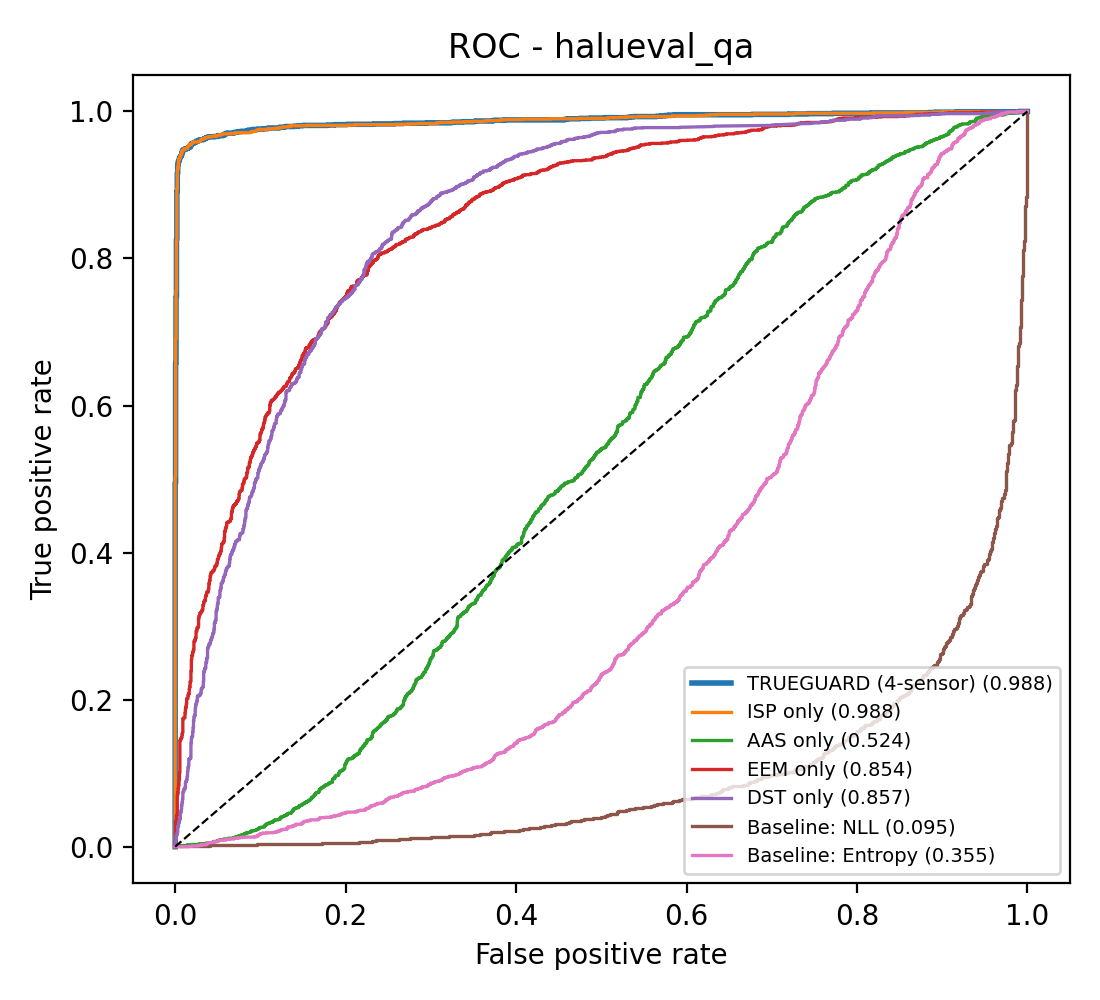
\includegraphics[width=\linewidth]{figures/Fig5a_ROC_HaluEval_QA.png}
\end{minipage}\hfill
\begin{minipage}{0.32\textwidth}
\centering
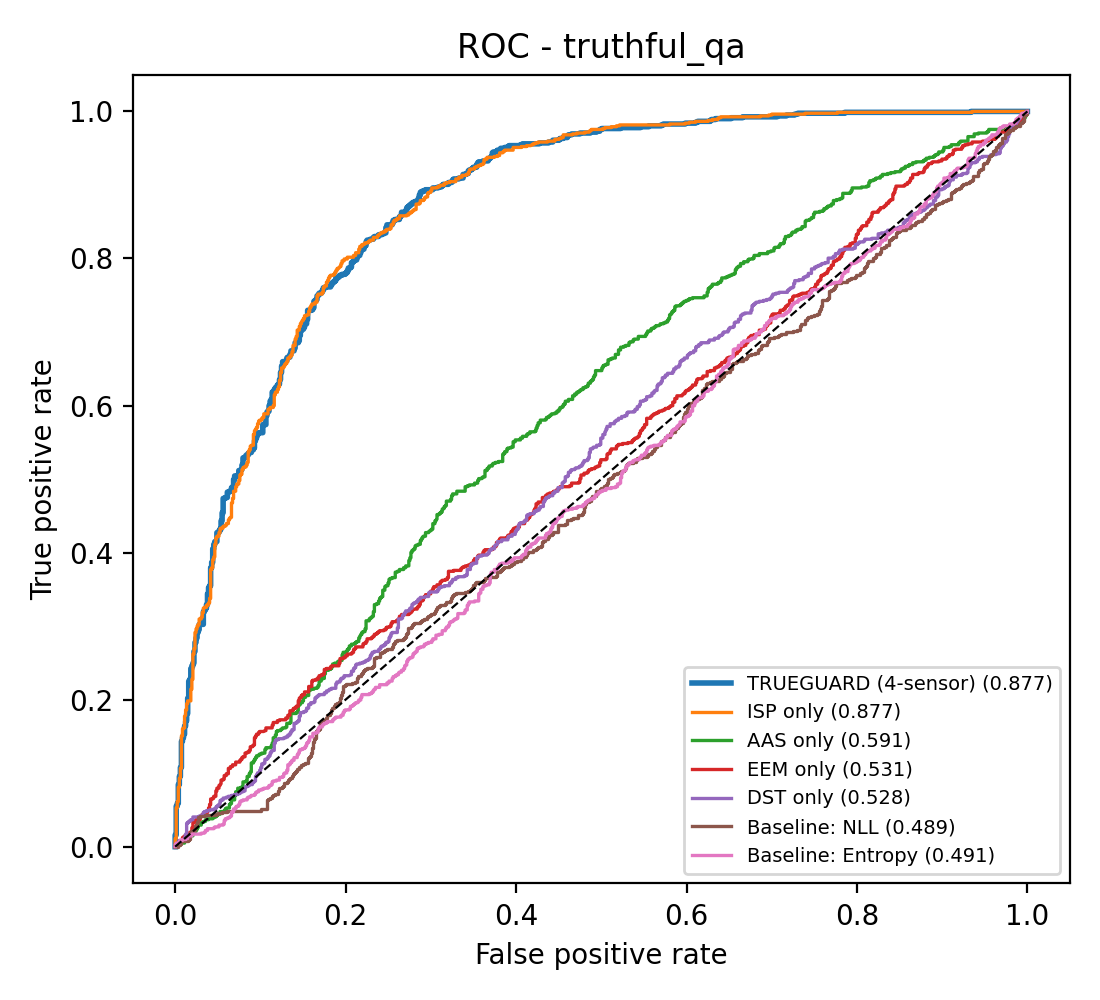
\includegraphics[width=\linewidth]{figures/Fig5b_ROC_TruthfulQA.png}
\end{minipage}\hfill
\begin{minipage}{0.32\textwidth}
\centering
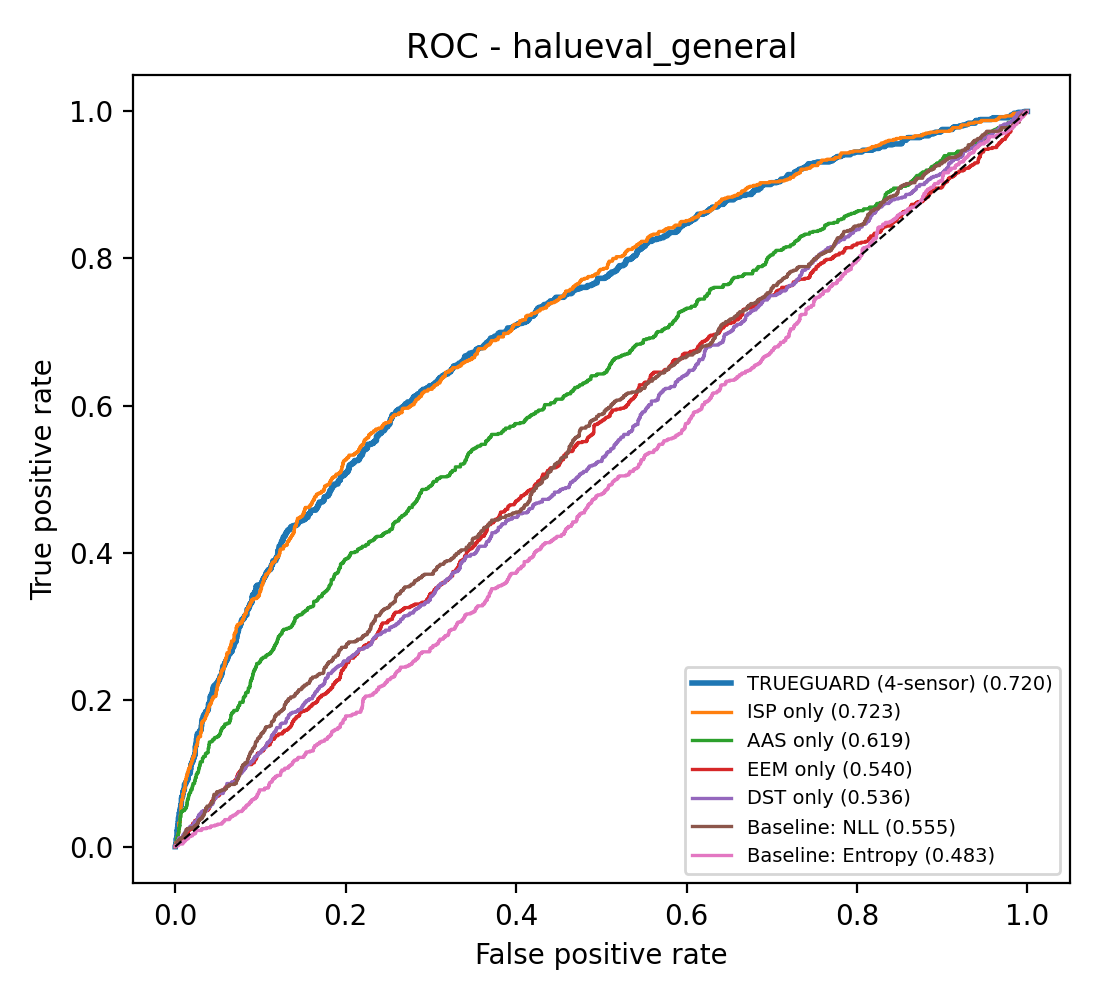
\includegraphics[width=\linewidth]{figures/Fig5c_ROC_HaluEval_General.png}
\end{minipage}
\caption{Representative in-domain 5-fold group-preserving ROC curves for TRUEGUARD and individual sensors on (left) HaluEval-QA, (center) TruthfulQA, and (right) HaluEval-General.}
\label{fig:rocs}
\end{figure*}

\subsection{Dataset-Artifact Controls}
To test whether surface cues explain these high in-domain scores, we evaluated 1D answer length, answer-text TF-IDF, shuffled labels, and strictly length-matched subsets on the same five benchmarks (Table~\ref{tab:indomain}). On HaluEval-QA, answer length alone reaches 0.9572 AUROC and answer-text TF-IDF reaches 0.9661; only 6.4\% of pairs (128 pairs, 256 rows) fall within two tokens in length. When restricted to those length-matched pairs (where raw length AUROC drops to 0.5516), TRUEGUARD declines by 19.8 points from 0.9880 to 0.7901. On HaluEval-Summarization, length is uninformative (0.4902), yet answer-text TF-IDF alone reaches 0.9539 on the full dataset and 0.9608 on length-matched pairs, showing strong lexical and stylistic differences between reference and synthetic hallucinated summaries. High raw AUROCs on HaluEval therefore do not by themselves establish generalizable factual error detection.

At the same time, the controls confirm real signal beyond simple length and surface n-grams. Shuffled-label AUROCs stay near chance (0.4894 to 0.5123), ruling out split leakage. TRUEGUARD outperforms answer-text TF-IDF on all five full datasets by +0.0219 to +0.0709 AUROC. Under strict length matching ($|\Delta L| \le 2$), TRUEGUARD significantly outperforms TF-IDF on all four paired benchmarks, with paired bootstrap gains of +0.0829 on HaluEval-Dialogue ($p = 0.0010$), +0.0461 on HaluEval-QA ($p = 0.0350$), +0.0331 on HaluEval-Summarization ($p = 0.0010$), and +0.0712 on TruthfulQA ($p = 0.0010$). Refitting TF-IDF strictly inside each length-matched subset produces similar scores (0.7072, 0.7322, 0.9586, and 0.7501). While these results show evidence beyond length and TF-IDF, other subtler benchmark artifacts may still remain.

\subsection{Four-Sensor Ablation Study}
To determine each sensor family's contribution, we performed leave-one-sensor-out ablations across all five in-domain datasets (Table~\ref{tab:ablation} and Fig.~\ref{fig:ablation}). Removing ISP causes large AUROC drops ranging from -0.0584 to -0.2709, whereas removing AAS, EEM, or DST changes in-domain AUROC by at most 0.0018. In the pooled source fusion classifier, standardized \texttt{ISP\_logit} receives weight +2.9353 (more than 96\% of total weight magnitude), while all six scalar sensor features have absolute weights at or below 0.0680. Four-sensor fusion therefore does not consistently outperform ISP alone in AUROC. The auxiliary sensors provide low-FPR unique detections, raising union Recall@10\% FPR from 0.348 to 0.529 (+18.1\%) on HaluEval-General, and supply an unsupervised fallback when ISP degrades under domain shift.

\begin{table*}[t]
\centering
\caption{Leave-One-Sensor-Out Ablation and Low-FPR Complementarity}
\label{tab:ablation}
\resizebox{\textwidth}{!}{%
\begin{tabular}{lcccccccc}
\toprule
Dataset & Full (4) & $-$ISP ($\Delta$) & $-$AAS ($\Delta$) & $-$EEM ($\Delta$) & $-$DST ($\Delta$) & ISP Rec@10\%FPR & Union Rec@10\%FPR & Unique AAS / EEM / DST \\
\midrule
\texttt{halueval\_dialogue} & 0.9218 & 0.7249 (-0.1968) & 0.9218 (0.0000) & 0.9220 (+0.0002) & 0.9219 (0.0000) & 0.778 & 0.817 & 0.005 / 0.015 / 0.015 \\
\texttt{halueval\_qa} & 0.9880 & 0.9296 (-0.0584) & 0.9880 (0.0000) & 0.9880 (-0.0001) & 0.9880 (0.0000) & 0.976 & 0.984 & 0.001 / 0.003 / 0.004 \\
\texttt{halueval\_summarization} & 0.9936 & 0.7233 (-0.2709) & 0.9935 (-0.0001) & 0.9936 (+0.0001) & 0.9936 (0.0000) & 0.987 & 0.990 & 0.002 / 0.001 / 0.001 \\
\texttt{truthful\_qa} & 0.8773 & 0.6073 (-0.2694) & 0.8772 (0.0000) & 0.8778 (+0.0005) & 0.8767 (-0.0006) & 0.575 & 0.640 & 0.015 / 0.006 / 0.032 \\
\texttt{halueval\_general} & 0.7204 & 0.6226 (-0.0981) & 0.7207 (+0.0003) & 0.7222 (+0.0018) & 0.7205 (+0.0001) & 0.348 & 0.529 & 0.066 / 0.049 / 0.054 \\
\bottomrule
\end{tabular}}
\end{table*}

\begin{figure}[t]
\centering
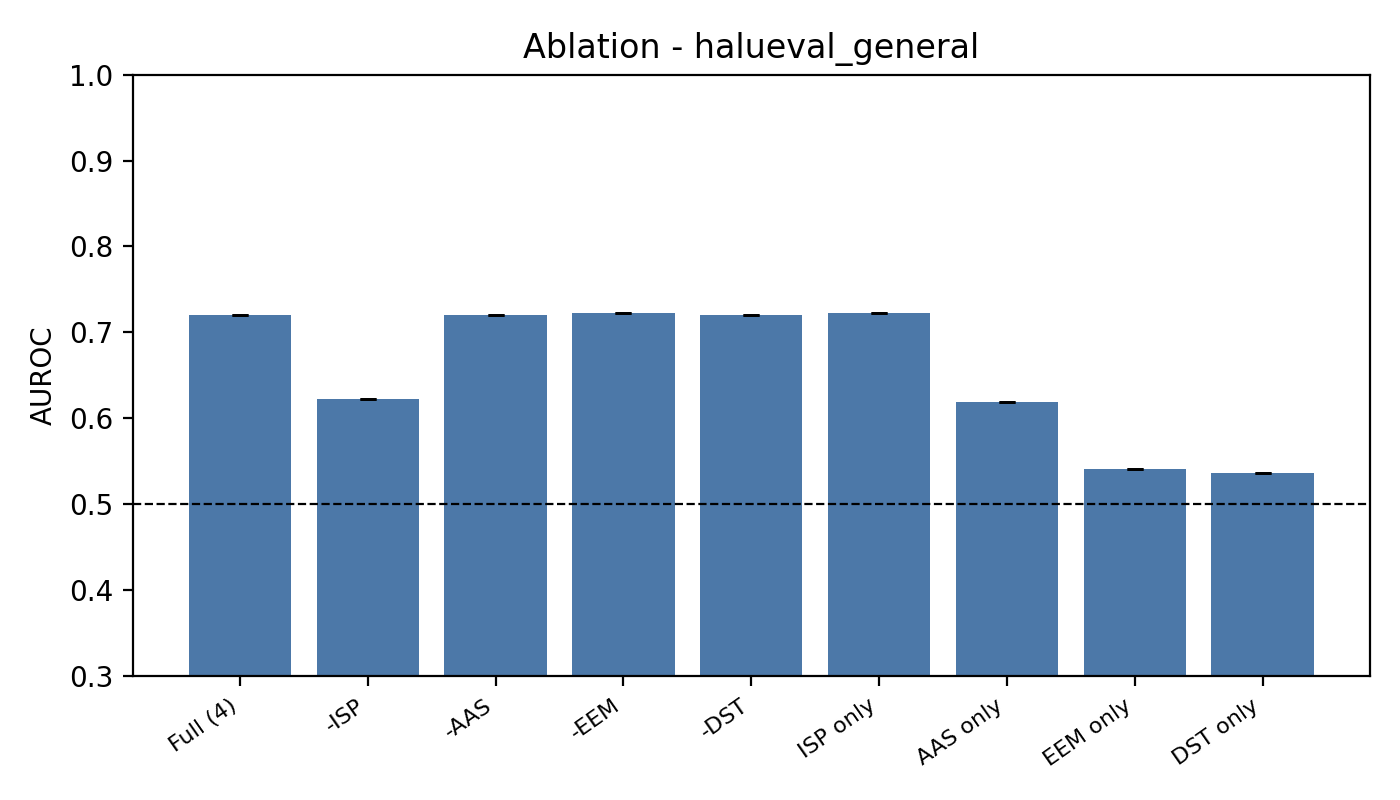
\includegraphics[width=\columnwidth]{figures/Fig6_Ablation_HaluEval_General.png}
\caption{Leave-one-sensor-out and single-sensor AUROC ablation on imbalanced HaluEval-General, showing AUROC across full four-sensor fusion, single-sensor removals ($-\text{ISP}$, $-\text{AAS}$, $-\text{EEM}$, $-\text{DST}$), and individual sensors (ISP, AAS, EEM, DST). Removing ISP produces the largest AUROC drop, while auxiliary-sensor low-FPR recall complementarity is reported in Table~\ref{tab:ablation}.}
\label{fig:ablation}
\end{figure}

\subsection{Zero-Shot Cross-Domain Performance}
To test whether pooled in-domain training transfers without target labels, we applied the pooled source detector unchanged to Datasets 6 through 9. Exact Colab \texttt{.npz} test AUROCs on the 40\% splits drop to near-chance across every target benchmark: 0.4929 on FaithDial, 0.4883 on WikiBio-GPT3, 0.4597 on XSum-Factuality, and 0.5205 on FEVER, accompanied by severe miscalibration (ECE from 0.3419 to 0.6574). A similar degradation appears off the diagonal of the in-domain 5-by-5 transfer matrix (Fig.~\ref{fig:transfer}). Yet frozen TinyLlama hidden states do retain target-domain linear separability: fitting 5-fold ISP probes directly on each target dataset achieves 0.8927 AUROC on FaithDial, 0.8754 on FEVER, 0.7427 on WikiBio-GPT3, and 0.6794 on XSum-Factuality. Zero-shot failure therefore reflects domain-dependent decision boundaries rather than an absence of useful information in the frozen representations.

\begin{figure}[t]
\centering
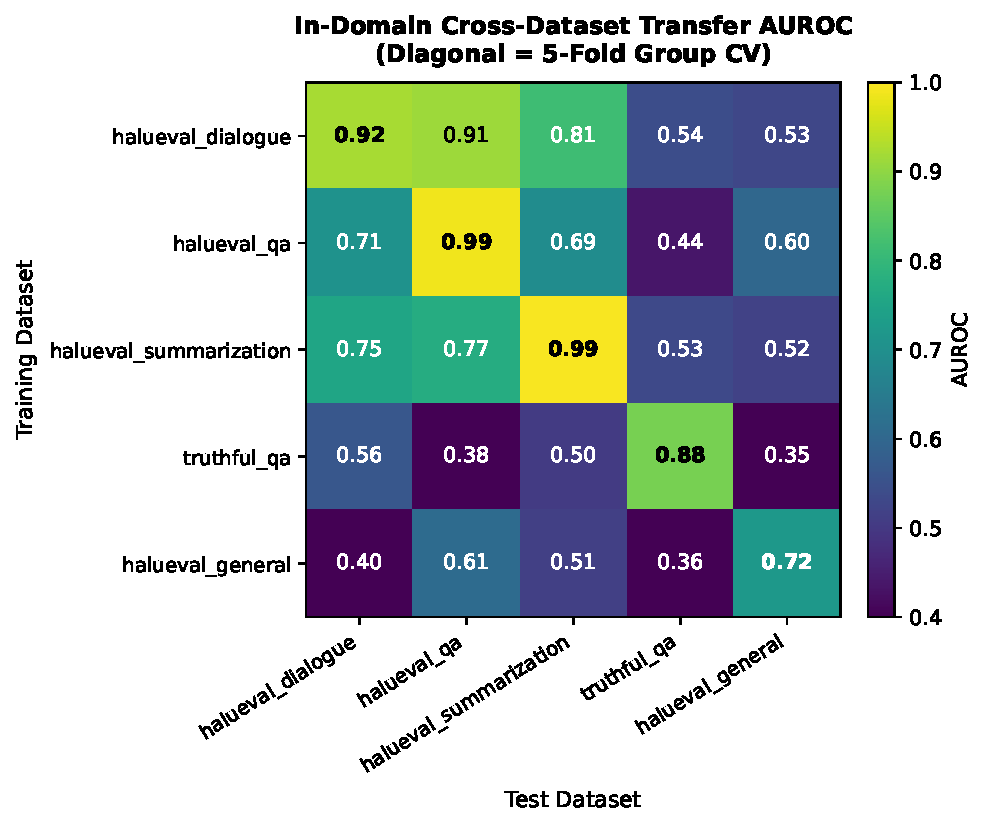
\includegraphics[width=\columnwidth]{figures/Fig4_InDomain_5x5_Transfer_Matrix_v2.pdf}
\caption{In-domain 5$\times$5 cross-dataset transfer AUROC matrix, showing strong diagonal 5-fold group cross-validation performance and off-diagonal degradation across tasks.}
\label{fig:transfer}
\end{figure}

\subsection{Target-Domain Few-Shot Refitting}
To measure how much target-domain supervision is needed to recover detection accuracy, we evaluated Target-Domain Few-Shot Refitting (Target-Only Probe Training) across $K \in \{50, 100, 250\}$ on identical 40\% group-disjoint test splits (Table~\ref{tab:fewshot} and Fig.~\ref{fig:fewshot}). Source Risk Recalibration (SrcRecal) stays near chance (0.4957 to 0.5242) across all four datasets and all $K$, confirming zero recoverable signal from pooled source probabilities.

At $K = 50$, simpler baselines outperform 2,048-dimensional target-only TRUEGUARD probes on every dataset: 1D EEM leads on FaithDial (0.7473 vs.\ 0.6987) and XSum-Factuality (0.6082 vs.\ 0.5401), while answer-text TF-IDF leads on WikiBio-GPT3 (0.5321 vs.\ 0.5088) and FEVER (0.5699 vs.\ 0.5394). At $K = 250$ (under 2~s CPU per refit), gains are task-dependent. Target-only TRUEGUARD clearly outperforms all simple baselines on FaithDial (0.8231, +0.0758 over 1D EEM and +0.1616 over TF-IDF), FEVER (0.7325, +0.1010 over TF-IDF), and WikiBio-GPT3 (0.6698, +0.0595 over TF-IDF), while reducing ECE by 82\% to 93\%. On XSum-Factuality, however, target-only TRUEGUARD (0.6456) approximately matches the 1D answer-length baseline (0.6445), offering no practical gain over length alone.

\begin{table*}[t]
\centering
\caption{Target-Domain Few-Shot Refitting (Target-Only Probe Training) vs.\ Source Recalibration and Simple Baselines}
\label{tab:fewshot}
\resizebox{\textwidth}{!}{%
\begin{tabular}{lcccccccc}
\toprule
Target Dataset (40\% Test) & ZS Exact & $K$ & Target-Only TG (10 seeds) & Source Risk Recal. & 1D EEM Cal. & 1D Length (LEN) & Answer TF-IDF & $K{=}250$ ECE (ZS) \\
\midrule
\texttt{faithdial} & 0.4929 & 50 & 0.6987 $\pm$ 0.0881 & 0.4957 $\pm$ 0.0060 & \textbf{0.7473} $\pm$ 0.0000 & 0.6721 $\pm$ 0.0000 & 0.5818 $\pm$ 0.0406 & N/A \\
\texttt{faithdial} & 0.4929 & 100 & \textbf{0.7899} $\pm$ 0.0313 & 0.5029 $\pm$ 0.0069 & 0.7473 $\pm$ 0.0000 & 0.6721 $\pm$ 0.0000 & 0.6145 $\pm$ 0.0249 & N/A \\
\texttt{faithdial} & 0.4929 & 250 & \textbf{0.8231} $\pm$ 0.0121 & 0.5043 $\pm$ 0.0060 & 0.7473 $\pm$ 0.0000 & 0.6721 $\pm$ 0.0000 & 0.6615 $\pm$ 0.0187 & \textbf{0.0443} (0.6574) \\
\midrule
\texttt{wikibio\_gpt3} & 0.4883 & 50 & 0.5088 $\pm$ 0.0562 & 0.4977 $\pm$ 0.0121 & 0.5000 $\pm$ 0.0235 & 0.4909 $\pm$ 0.0470 & \textbf{0.5321} $\pm$ 0.0274 & N/A \\
\texttt{wikibio\_gpt3} & 0.4883 & 100 & 0.4939 $\pm$ 0.0840 & 0.4977 $\pm$ 0.0121 & 0.5045 $\pm$ 0.0231 & 0.4727 $\pm$ 0.0384 & \textbf{0.5785} $\pm$ 0.0395 & N/A \\
\texttt{wikibio\_gpt3} & 0.4883 & 250 & \textbf{0.6698} $\pm$ 0.0381 & 0.5023 $\pm$ 0.0121 & 0.4955 $\pm$ 0.0231 & 0.4909 $\pm$ 0.0470 & 0.6103 $\pm$ 0.0290 & \textbf{0.0737} (0.4336) \\
\midrule
\texttt{xsum\_factuality} & 0.4597 & 50 & 0.5401 $\pm$ 0.0686 & 0.5000 $\pm$ 0.0425 & \textbf{0.6082} $\pm$ 0.0855 & 0.5867 $\pm$ 0.1218 & 0.5329 $\pm$ 0.0457 & N/A \\
\texttt{xsum\_factuality} & 0.4597 & 100 & 0.6058 $\pm$ 0.0430 & 0.5242 $\pm$ 0.0340 & 0.6352 $\pm$ 0.0000 & \textbf{0.6445} $\pm$ 0.0000 & 0.5331 $\pm$ 0.0370 & N/A \\
\texttt{xsum\_factuality} & 0.4597 & 250 & \textbf{0.6456} $\pm$ 0.0410 & 0.5161 $\pm$ 0.0389 & 0.6352 $\pm$ 0.0000 & \textbf{0.6445} $\pm$ 0.0000 & 0.5456 $\pm$ 0.0323 & \textbf{0.0383} (0.5629) \\
\midrule
\texttt{fever} (claim verif.) & 0.5205 & 50 & 0.5394 $\pm$ 0.0482 & 0.5123 $\pm$ 0.0173 & 0.5176 $\pm$ 0.0425 & 0.4977 $\pm$ 0.0117 & \textbf{0.5699} $\pm$ 0.0183 & N/A \\
\texttt{fever} (claim verif.) & 0.5205 & 100 & \textbf{0.6195} $\pm$ 0.0395 & 0.5000 $\pm$ 0.0216 & 0.5264 $\pm$ 0.0371 & 0.4955 $\pm$ 0.0110 & 0.5966 $\pm$ 0.0224 & N/A \\
\texttt{fever} (claim verif.) & 0.5205 & 250 & \textbf{0.7325} $\pm$ 0.0136 & 0.5000 $\pm$ 0.0216 & 0.5264 $\pm$ 0.0371 & 0.5045 $\pm$ 0.0110 & 0.6315 $\pm$ 0.0104 & \textbf{0.0430} (0.3419) \\
\bottomrule
\end{tabular}}
\end{table*}

\begin{figure*}[t]
\centering
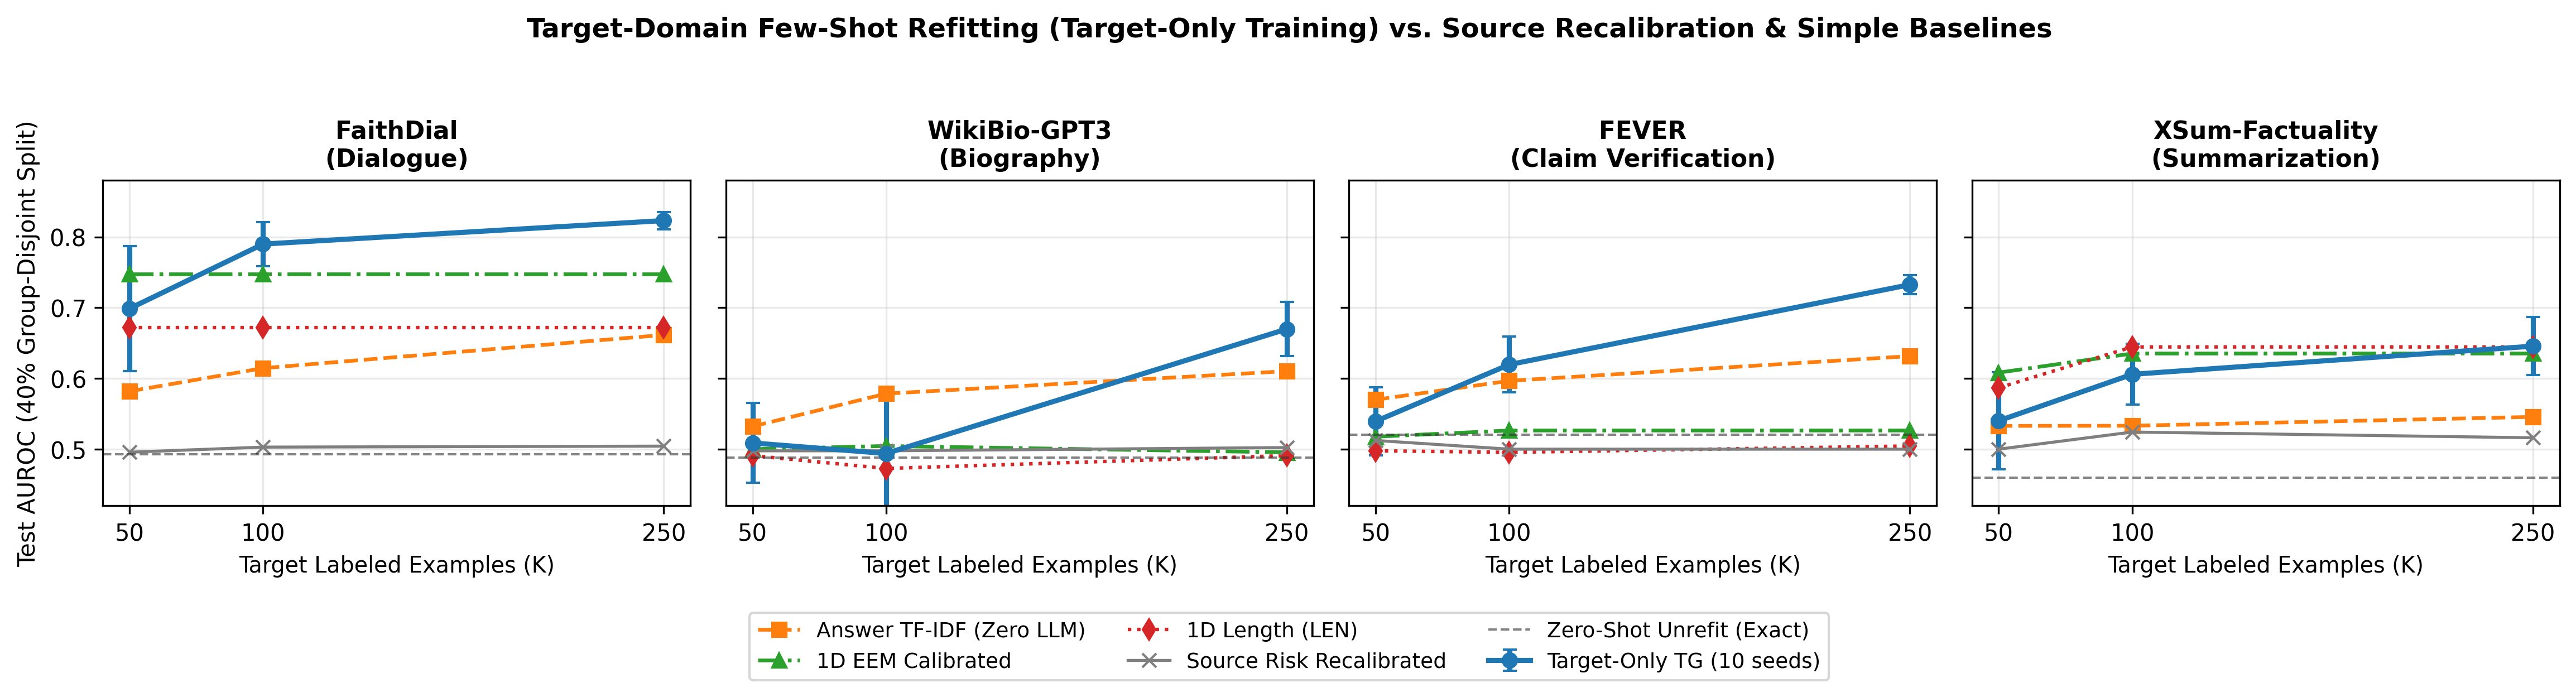
\includegraphics[width=\textwidth]{figures/Fig2_TargetDomain_FewShot_Refitting_vs_Baselines.png}
\caption{Target-domain few-shot refitting ($K = 50, 100, 250$, 10 seeds) compared with zero-shot unrefitted TRUEGUARD, source risk recalibration, 1D EEM, 1D LEN, and answer-text TF-IDF across four group-disjoint 40\% test sets.}
\label{fig:fewshot}
\end{figure*}

\subsection{Cross-Domain Probe Diagnostics}
To examine why linear probes fail to transfer across domains, we compared within-domain split-half probe weight cosines against cross-domain cosines (Table~\ref{tab:diag} and Fig.~\ref{fig:diag}(a)). Because random vectors in 2,048 dimensions have a cosine similarity standard deviation of 0.0221, a within-domain baseline is necessary to interpret small cross-domain values. On full datasets, within-domain split-half cosines range from +0.2300 to +0.6888 on homogeneous benchmarks (10 to 31 times the random standard deviation), whereas cross-domain cosines against the pooled source probe lie between -0.0306 and +0.0510.

To remove sample-size differences across datasets, we repeated this analysis at strictly equal sample size ($N_{\text{fit}} = 900$ per half across three seeds and four layers). Within-domain cosines remain substantially above zero, from +0.1125 on XSum-Factuality to +0.6707 on HaluEval-Summarization, whereas cross-domain cosines from HaluEval to each unseen target remain centered near zero (-0.0151 on FaithDial, +0.0032 on WikiBio-GPT3, +0.0204 on FEVER, and +0.0092 on XSum-Factuality). Because L2-regularized linear coefficients in correlated 2,048-dimensional spaces are not uniquely identifiable causal directions, we treat this contrast strictly as empirical diagnostic evidence of domain-dependent linear decision boundaries.

\begin{table*}[t]
\centering
\caption{Empirical Domain-Shift Diagnostics: Probe Alignment and Length-Controlled EEM}
\label{tab:diag}
\resizebox{\textwidth}{!}{%
\begin{tabular}{lccccccc}
\toprule
Dataset & Within-Domain Cos (Full) & Within-Domain Cos ($N{=}900$) & Cross-Domain Cos (Pool / $N{=}900$) & Raw $\text{EEM}_{\text{mean}}$ & $\rho(\text{EEM}, \text{LEN})$ & Quartile Mean EEM & LM ($|\Delta L|\le 2$) EEM \\
\midrule
\texttt{halueval\_summarization} & +0.6888 $\pm$ 0.0132 & +0.6707 $\pm$ 0.0129 & Source & 0.5787 & -0.0658 & 0.5331 & 0.5770 \\
\texttt{halueval\_qa} & +0.4358 $\pm$ 0.0246 & +0.4999 $\pm$ 0.0363 & Source & \textbf{0.3627} & \textbf{-0.2909} & 0.4465 & \textbf{0.5184} \\
\texttt{halueval\_dialogue} & +0.3929 $\pm$ 0.0379 & +0.3930 $\pm$ 0.0280 & Source & \textbf{0.3740} & -0.1038 & \textbf{0.3795} & \textbf{0.4525} \\
\texttt{truthful\_qa} & +0.3440 $\pm$ 0.0269 & N/A & Source & 0.4912 & -0.3678 & 0.4720 & 0.5030 \\
\texttt{halueval\_general} & +0.0506 $\pm$ 0.0252 & N/A & Source & 0.4829 & -0.1637 & 0.4545 & N/A \\
\texttt{fever} & +0.3680 $\pm$ 0.0212 & +0.2668 $\pm$ 0.0189 & +0.0510 / +0.0204 & 0.5417 & -0.4285 & 0.5547 & N/A \\
\texttt{faithdial} & +0.2300 $\pm$ 0.0206 & +0.2205 $\pm$ 0.0168 & -0.0306 / -0.0151 & \textbf{0.7456} & \textbf{+0.0058} & \textbf{0.7662} & N/A \\
\texttt{wikibio\_gpt3} & +0.1290 $\pm$ 0.0224 & +0.1282 $\pm$ 0.0318 & -0.0045 / +0.0032 & 0.5207 & -0.2348 & 0.5278 & N/A \\
\texttt{xsum\_factuality} & +0.1073 $\pm$ 0.0272 & +0.1125 $\pm$ 0.0295 & +0.0280 / +0.0092 & \textbf{0.6648} & \textbf{-0.0321} & \textbf{0.6648} & N/A \\
\midrule
\textit{Random 2048-d Null} & \textit{0.0000 $\pm$ 0.0221} & \textit{0.0000 $\pm$ 0.0221} & \textit{0.0000 $\pm$ 0.0221} & \textit{0.5000} & \textit{0.0000} & \textit{0.5000} & \textit{0.5000} \\
\bottomrule
\end{tabular}}
\end{table*}

\begin{figure*}[t]
\centering
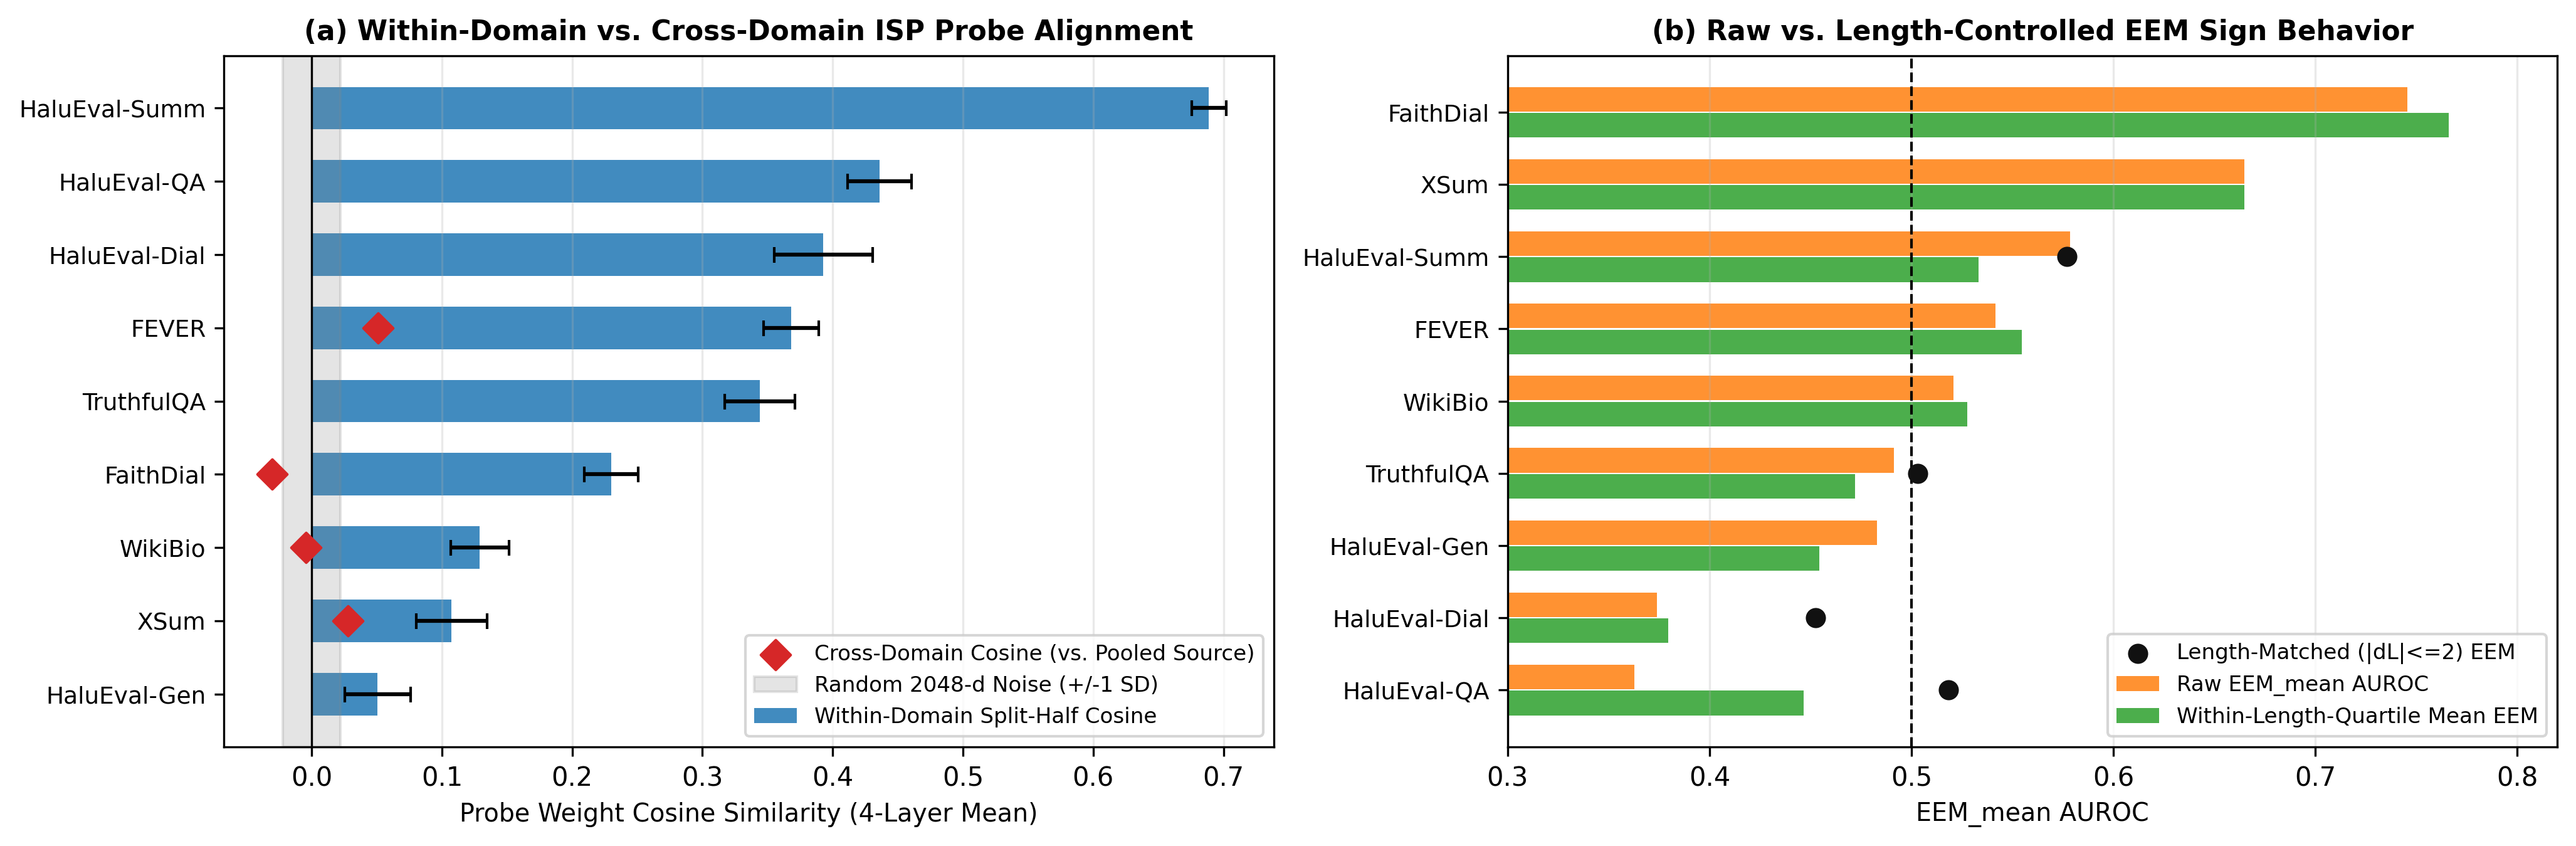
\includegraphics[width=\textwidth]{figures/Fig8_CrossDomain_Diagnostics_Cosine_and_LengthControlled_EEM.png}
\caption{Empirical domain-shift diagnostics: (a) within-domain split-half vs.\ cross-domain ISP probe weight cosine similarity relative to the 2,048-d random noise band; (b) raw vs.\ length-controlled $\text{EEM}_{\text{mean}}$ AUROC across nine benchmarks.}
\label{fig:diag}
\end{figure*}

\subsection{Length-Controlled Entropy Analysis}
Raw unsupervised sensor AUROCs across the nine teacher-forced benchmarks (Fig.~\ref{fig:signinv}) show opposite EEM directions on synthetic HaluEval (0.3627 on QA, 0.3740 on Dialogue) versus natural FaithDial (0.7456) and XSum-Factuality (0.6648). To test whether answer length confounds this pattern, we computed $\text{EEM}_{\text{mean}}$ AUROC within four length quartiles and on length-matched pairs (Table~\ref{tab:diag} and Fig.~\ref{fig:diag}(b)). Three distinct behaviors emerge. On FaithDial ($\rho = +0.0058$, quartile-mean 0.7662) and XSum-Factuality ($\rho = -0.0321$, quartile-mean 0.6648), positive EEM signal persists unchanged after length control. On HaluEval-QA, $\text{EEM}_{\text{mean}}$ correlates negatively with length ($\rho = -0.2909$), and length matching removes the apparent inversion (0.3627 to 0.5184). On HaluEval-Dialogue, however, the inverse association persists within length quartiles (0.3795) and partially under length matching (0.4525).

\begin{figure}[t]
\centering
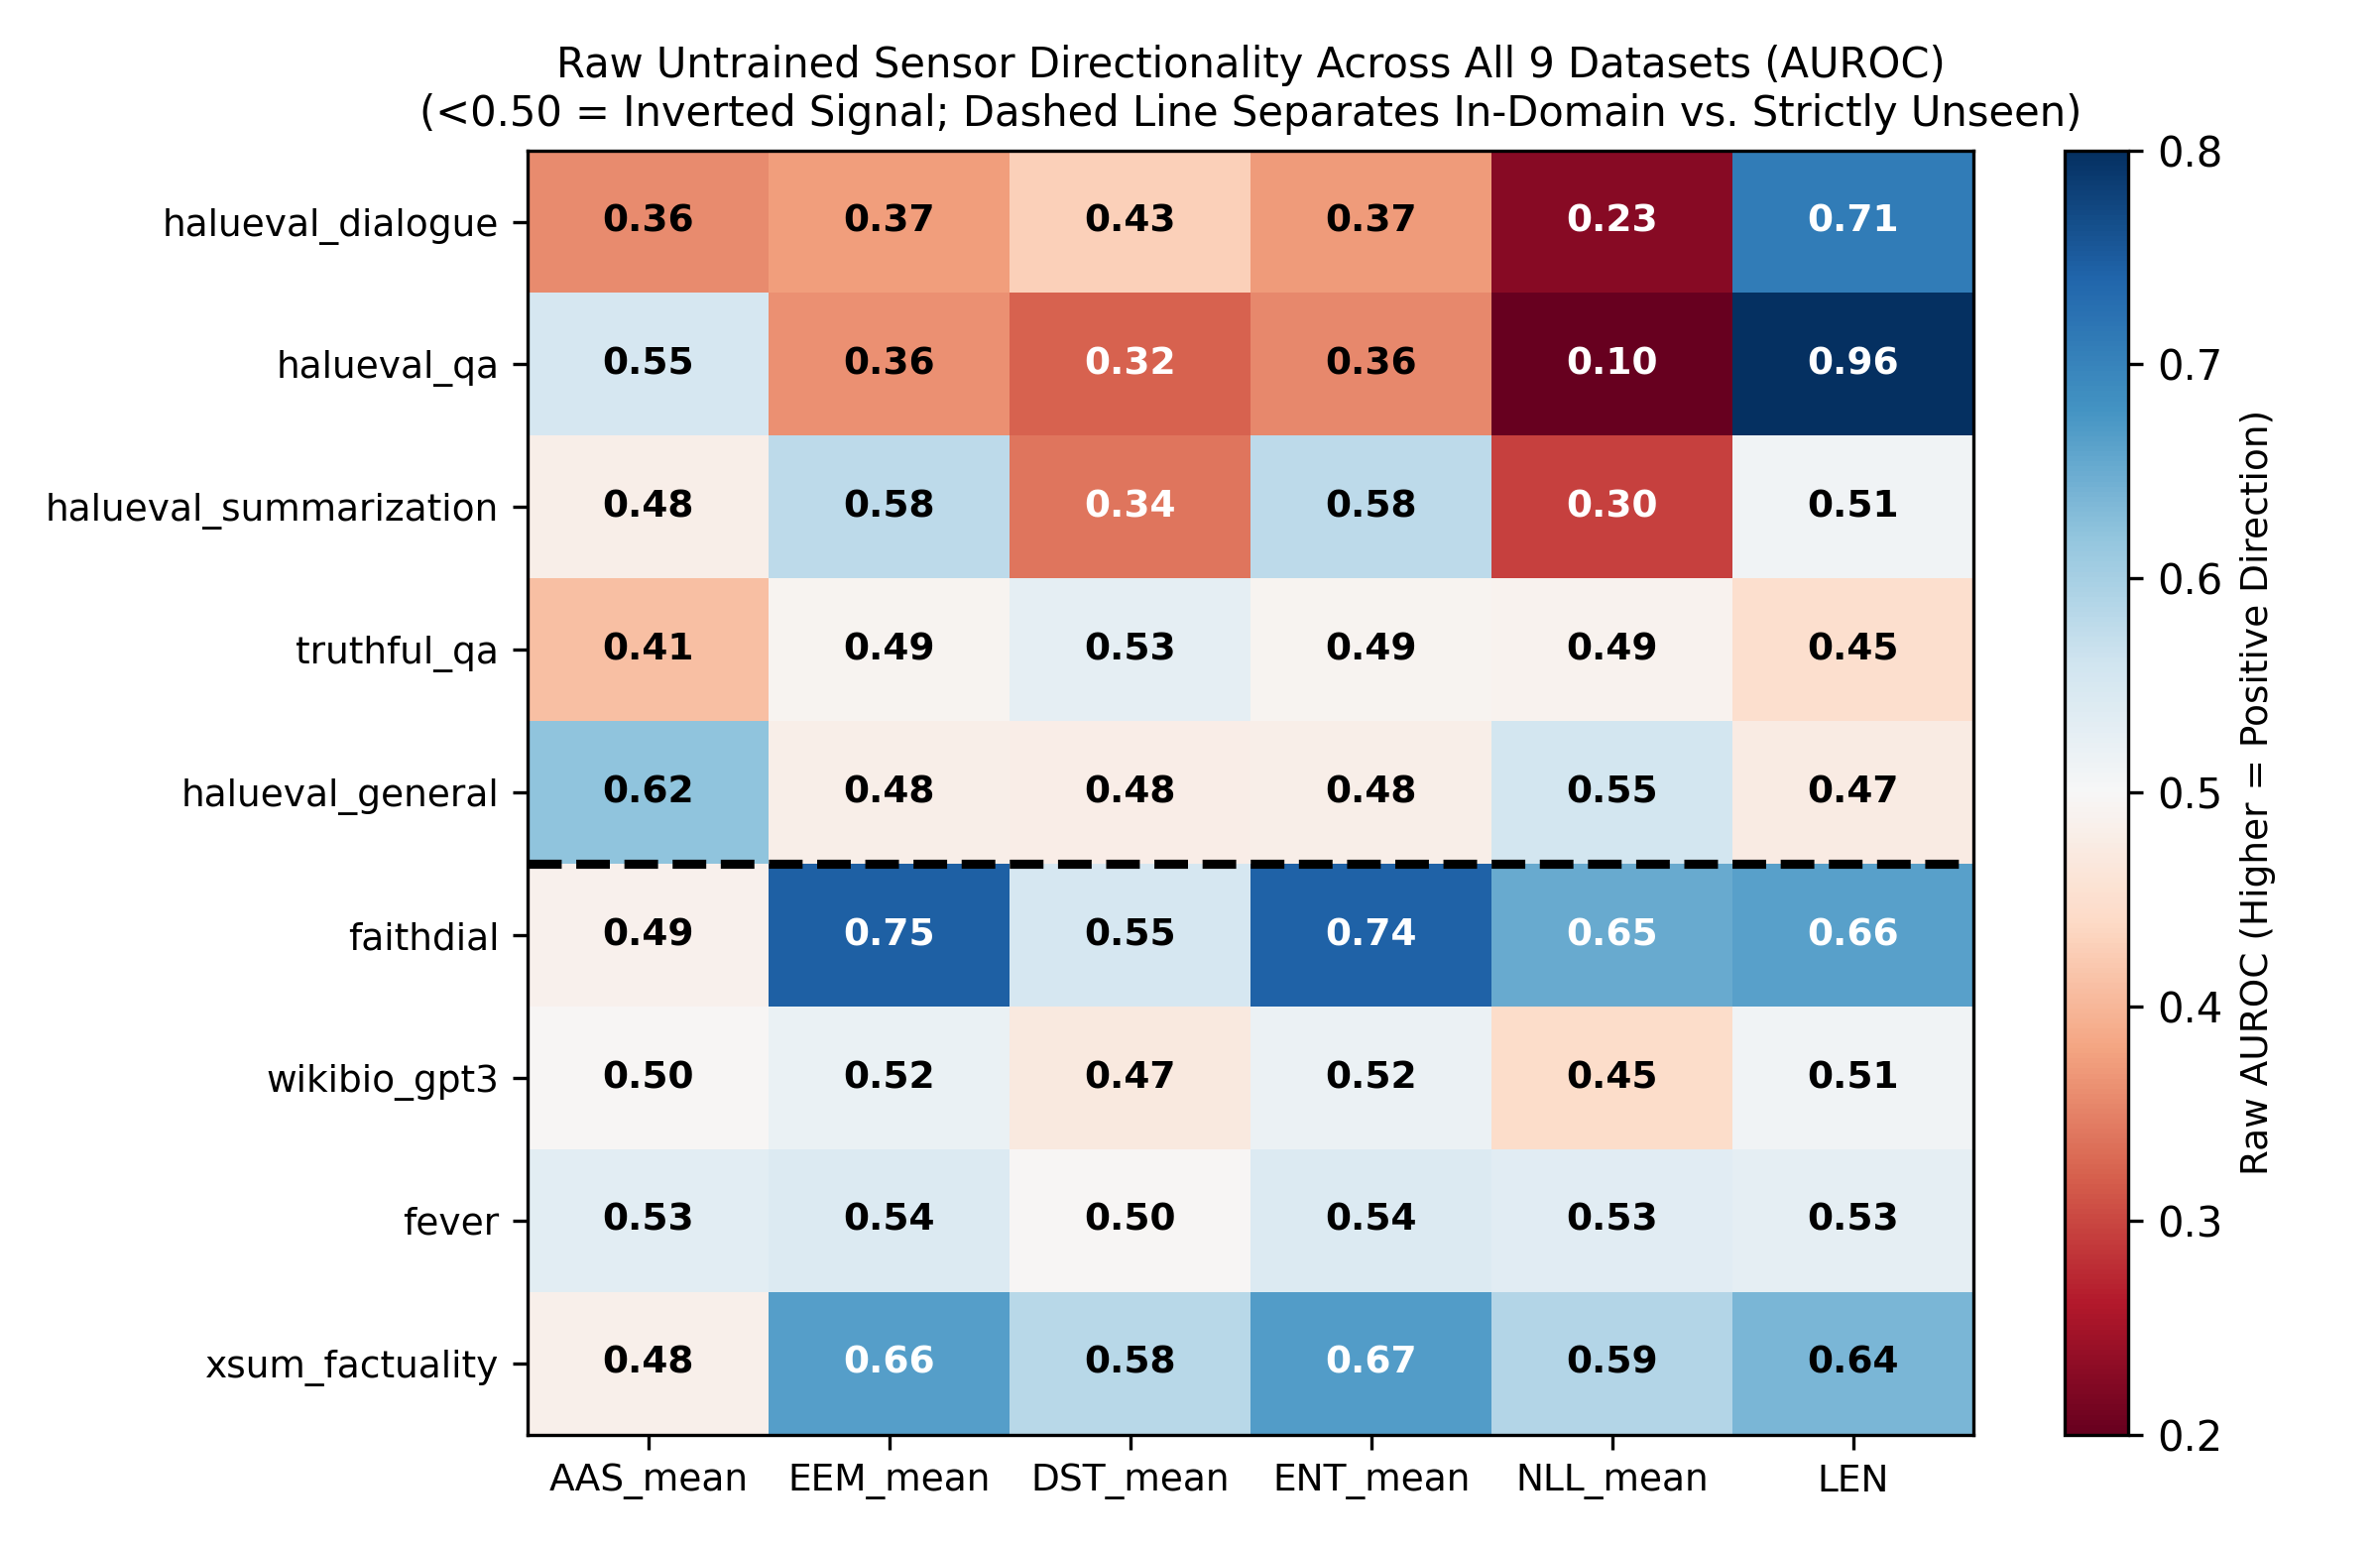
\includegraphics[width=\columnwidth]{figures/Fig1_Sensor_Sign_Inversion_9Datasets.png}
\caption{Raw unsupervised sensor AUROCs across nine teacher-forced benchmarks, illustrating domain-dependent signal polarity between synthetic HaluEval and natural dialogue/summarization datasets.}
\label{fig:signinv}
\end{figure}

\subsection{Comparison With Existing Detection Methods}
To benchmark TRUEGUARD against established detectors on TinyLlama's own generations, we evaluated all methods on the same 250 held-out TriviaQA test questions (Table~\ref{tab:external} and Fig.~\ref{fig:external}). Target-refitted single-pass \texttt{TRUEGUARD\_4sensor} ($K = 250$ calibration labels) reaches 0.7876 AUROC (95\% CI [0.720, 0.852]) and 0.4360 AURC ([0.360, 0.523]). Under these different supervision settings, it significantly outperforms label-free 10-sample \texttt{Semantic\_Entropy\_LN} (0.6859 AUROC, $p_{\text{Holm}} = 0.012$; 0.5411 AURC, $p_{\text{Holm}} = 0.006$), \texttt{Semantic\_Entropy\_Disc} (0.6856 AUROC, $p_{\text{Holm}} = 0.012$), \texttt{Predictive\_Entropy} (0.6583 AUROC, $p_{\text{Holm}} = 0.006$), and \texttt{NLL} (0.4678 AUROC, $p_{\text{Holm}} = 0.006$). Against label-free 10-sample \texttt{SelfCheckGPT\_NLI} (0.7477 AUROC, 0.4659 AURC, 0.8537 AUPRC), TRUEGUARD's observed AUROC (+0.0399) and AURC (-0.0299) differences are not statistically significant ($p_{\text{Holm}} = 0.478$ and $0.362$), while SelfCheckGPT-NLI obtains slightly higher AUPRC (0.8537 vs.\ 0.8460).

Supervision plays a decisive role in this result. Without TriviaQA labels, \texttt{TRUEGUARD\_Pooled\_ZS} drops to 0.5504 AUROC and 0.6342 AURC, falling below every label-free baseline except NLL. In addition, forensic inspection confirmed that NLL's below-chance AUROC of 0.4678 (95\% CI [0.396, 0.542]) is a genuine observation rather than a sign or orientation bug: all 250 NLL values are non-negative, NLL correlates positively with predictive entropy ($r = +0.6698$), and TinyLlama-1.1B assigns slightly lower mean NLL to fluent hallucinated answers ($0.7711 \pm 0.2003$) than to terse correct factual entities ($0.7991 \pm 0.2370$).

\begin{table*}[t]
\centering
\caption{Head-to-Head Comparison Against External Baselines on Identical 250 TriviaQA Test Questions (Supervision-Distinguished)}
\label{tab:external}
\resizebox{\textwidth}{!}{%
\begin{tabular}{llclccccccc}
\toprule
Method ($n_{\text{cal}}{=}250, n_{\text{test}}{=}250$) & Supervision / Target Labels & Gens/Q & Extra Model & AUROC [95\% CI] & AUPRC & F1 (Cal) & AURC [95\% CI] & Acc@46\% & $\Delta$AUROC ($p_{\text{Holm}}$) & $\Delta$AURC ($p_{\text{Holm}}$) \\
\midrule
\textbf{TRUEGUARD\_4sensor} & Supervised (250 cal) & 1 & None & \textbf{0.7876} [0.720, 0.852] & 0.8460 & \textbf{0.8084} & \textbf{0.4360} [0.360, 0.523] & \textbf{55.6\%} & N/A & N/A \\
\textbf{TRUEGUARD\_ISP\_only} & Supervised (250 cal) & 1 & None & 0.7706 [0.701, 0.834] & 0.8476 & 0.8062 & 0.4473 [0.369, 0.532] & 53.9\% & +0.0170 (0.478) & -0.0113 (0.451) \\
\textbf{TRUEGUARD\_Pooled\_ZS} & Zero-Shot (0 target) & 1 & None & 0.5504 & 0.7124 & N/A & 0.6342 & 37.4\% & +0.2372 & -0.1982 \\
\textbf{SelfCheckGPT\_NLI} & Label-Free (0 rank; 250 thr) & 11 & DeBERTa-v3-L & 0.7477 [0.681, 0.812] & \textbf{0.8537} & 0.5920 & 0.4659 [0.385, 0.559] & 50.4\% & +0.0399 (0.478) & -0.0299 (0.362) \\
\textbf{Semantic\_Entropy\_LN} & Label-Free (0 rank; 250 thr) & 10 & DeBERTa-L & 0.6859 [0.621, 0.756] & 0.8059 & 0.6377 & 0.5411 [0.450, 0.627] & 49.6\% & \textbf{+0.1017 (0.012)} & \textbf{-0.1051 (0.006)} \\
\textbf{Semantic\_Entropy\_Disc} & Label-Free (0 rank; 250 thr) & 10 & DeBERTa-L & 0.6856 [0.620, 0.753] & 0.8025 & 0.6403 & 0.5414 [0.452, 0.629] & 48.7\% & \textbf{+0.1020 (0.012)} & \textbf{-0.1054 (0.006)} \\
\textbf{Predictive\_Entropy} & Label-Free (0 rank; 250 thr) & 1 & None & 0.6583 [0.587, 0.730] & 0.7471 & 0.5985 & 0.5309 [0.448, 0.617] & 45.2\% & \textbf{+0.1293 (0.006)} & \textbf{-0.0949 (0.006)} \\
\textbf{NLL (Length-Norm.)} & Label-Free (0 rank; 250 thr) & 1 & None & 0.4678 [0.396, 0.542] & 0.6453 & 0.5423 & 0.6843 [0.603, 0.760] & 31.3\% & \textbf{+0.3198 (0.006)} & \textbf{-0.2483 (0.006)} \\
\bottomrule
\end{tabular}}
\end{table*}

\begin{figure}[t]
\centering
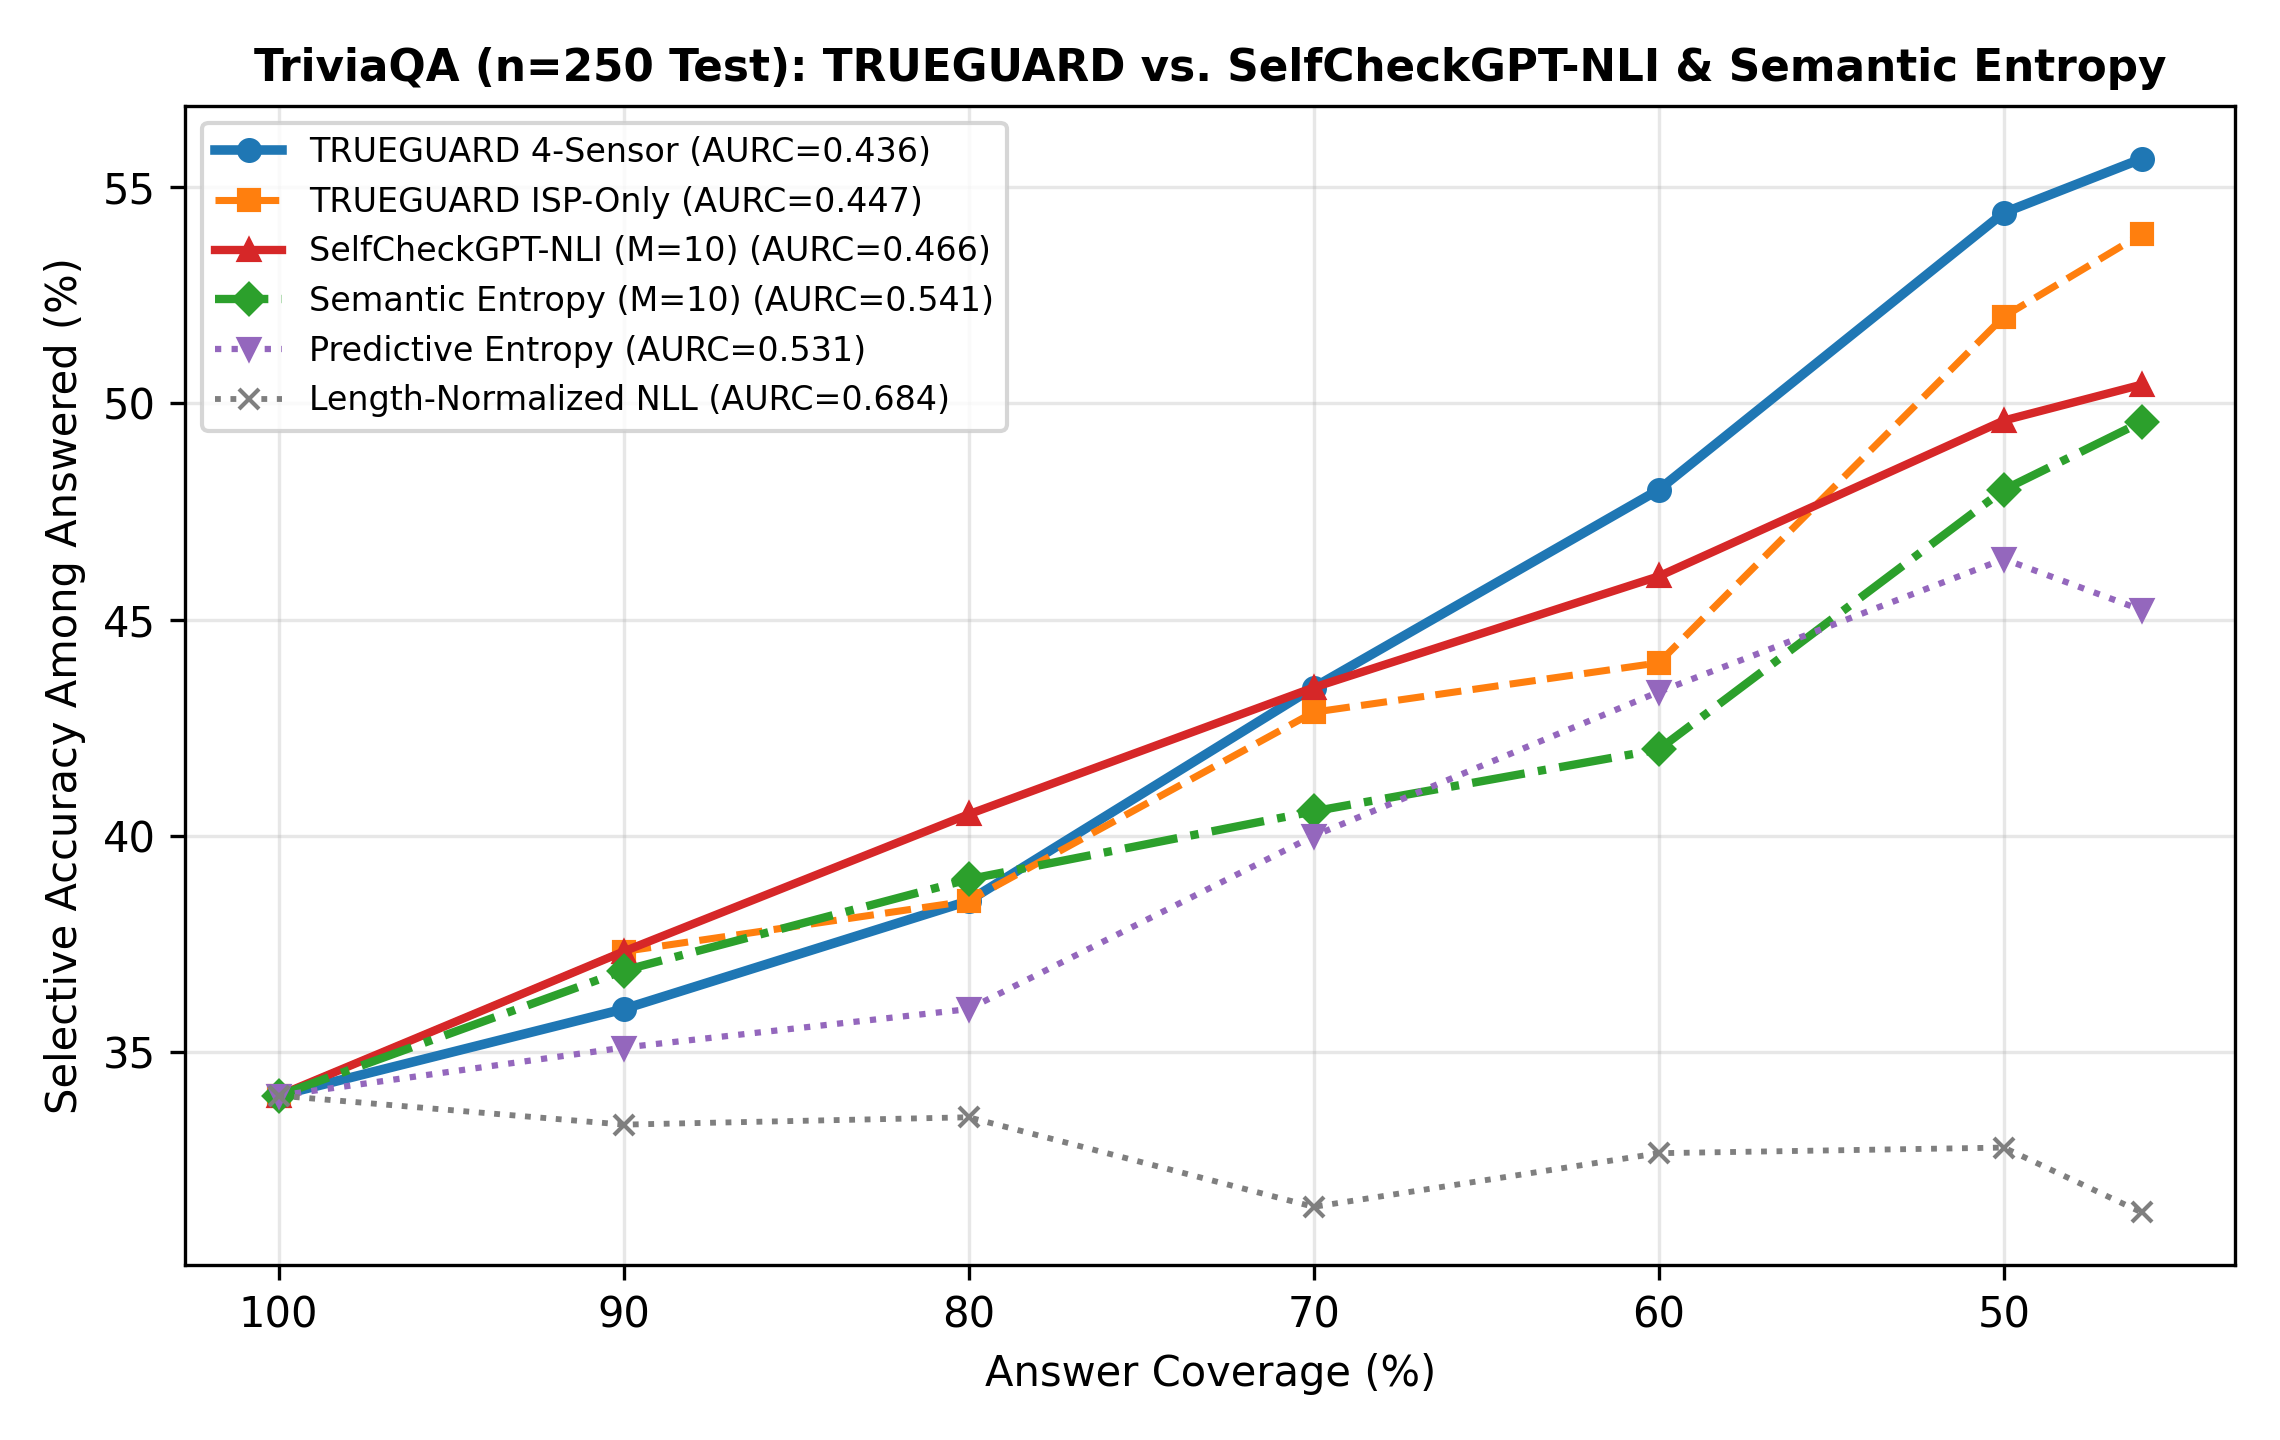
\includegraphics[width=\columnwidth]{figures/Fig7_External_Baselines_RiskCurve.png}
\caption{Risk-coverage selective prediction curves on the 250 held-out TriviaQA test questions comparing target-refitted TRUEGUARD with label-free SelfCheckGPT-NLI, Semantic Entropy, Predictive Entropy, and NLL.}
\label{fig:external}
\end{figure}

\subsection{Selective Prediction and Abstention}
To isolate the source of mitigation gains on closed-book TriviaQA (baseline greedy accuracy 34.00\%, hallucination rate 66.00\%), we compared pure selective abstention against the full three-tier controller at matched 46.0\% answer coverage (115 answered out of 250 questions; Table~\ref{tab:mitigation} and Fig.~\ref{fig:triviaqa_abstain}). Pure abstain-only selection, which simply answers the 115 lowest-risk questions, achieves 64 correct answers out of 115 (55.65\% selective accuracy), reducing system-wide incorrect outputs from 66.00\% to 20.40\%. The full three-tier controller (81 Safe, 23 Tier-1 Resample, 11 Tier-2 Wikipedia Retrieval, and 135 Tier-3 Abstain) achieves 63 correct answers out of 115 (54.78\% selective accuracy, 20.80\% system-wide incorrect outputs). Active Tier 1 and Tier 2 interventions repaired four originally incorrect answers (two by resampling and two by Wikipedia retrieval) while changing three originally correct greedy answers into incorrect ones, yielding a difference of one question. No measurable benefit from the active intervention tiers was established on this test set, and risk-based selective abstention accounts for the demonstrated mitigation gain.

\begin{table*}[t]
\centering
\caption{TriviaQA Closed-Book Selective Abstention vs.\ Full Three-Tier Controller Intervention Ablation ($n_{\text{test}} = 250$)}
\label{tab:mitigation}
\resizebox{\textwidth}{!}{%
\begin{tabular}{llccccccc}
\toprule
System / Method & Role & AUROC & AURC [95\% CI] & Coverage & Correct / Ans. & Selective Acc. & Sys.\ Halluc. & Fixed / Broken \\
\midrule
Greedy Baseline & Unfiltered baseline & N/A & N/A & 100.0\% (250/250) & 85 / 250 & 34.00\% & 66.00\% & 0 / 0 \\
\textbf{TRUEGUARD Pure Abstain-Only} & \textbf{Primary selective abstention} & \textbf{0.7876} & \textbf{0.4360} [0.360, 0.524] & 46.0\% (115/250) & \textbf{64 / 115} & \textbf{55.65\%} & \textbf{20.40\%} & 0 / 0 \\
TRUEGUARD Full 3-Tier Controller & Intervention ablation (T1+T2+T3) & 0.7876 & Fixed pt & 46.0\% (115/250) & 63 / 115 & 54.78\% (-0.87\%) & 20.80\% & 4 fixed / 3 broken \\
TRUEGUARD ISP-Only (Abstain) & Single-sensor ablation & 0.7706 & 0.4473 [0.369, 0.532] & 46.0\% (115/250) & 62 / 115 & 53.91\% & 21.20\% & 0 / 0 \\
Scalars-Only (Abstain) & No-ISP ablation & 0.7130 & 0.4891 [0.404, 0.577] & 46.0\% (115/250) & 57 / 115 & 49.57\% & 23.20\% & 0 / 0 \\
Predictive Entropy (Abstain) & Uncertainty baseline & 0.6583 & 0.5309 [0.448, 0.617] & 46.0\% (115/250) & 52 / 115 & 45.22\% & 25.20\% & 0 / 0 \\
Length-Norm.\ NLL (Abstain) & Likelihood baseline & 0.4678 & 0.6843 [0.603, 0.760] & 46.0\% (115/250) & 36 / 115 & 31.30\% & 31.60\% & 0 / 0 \\
\bottomrule
\end{tabular}}
\end{table*}

\begin{figure}[t]
\centering
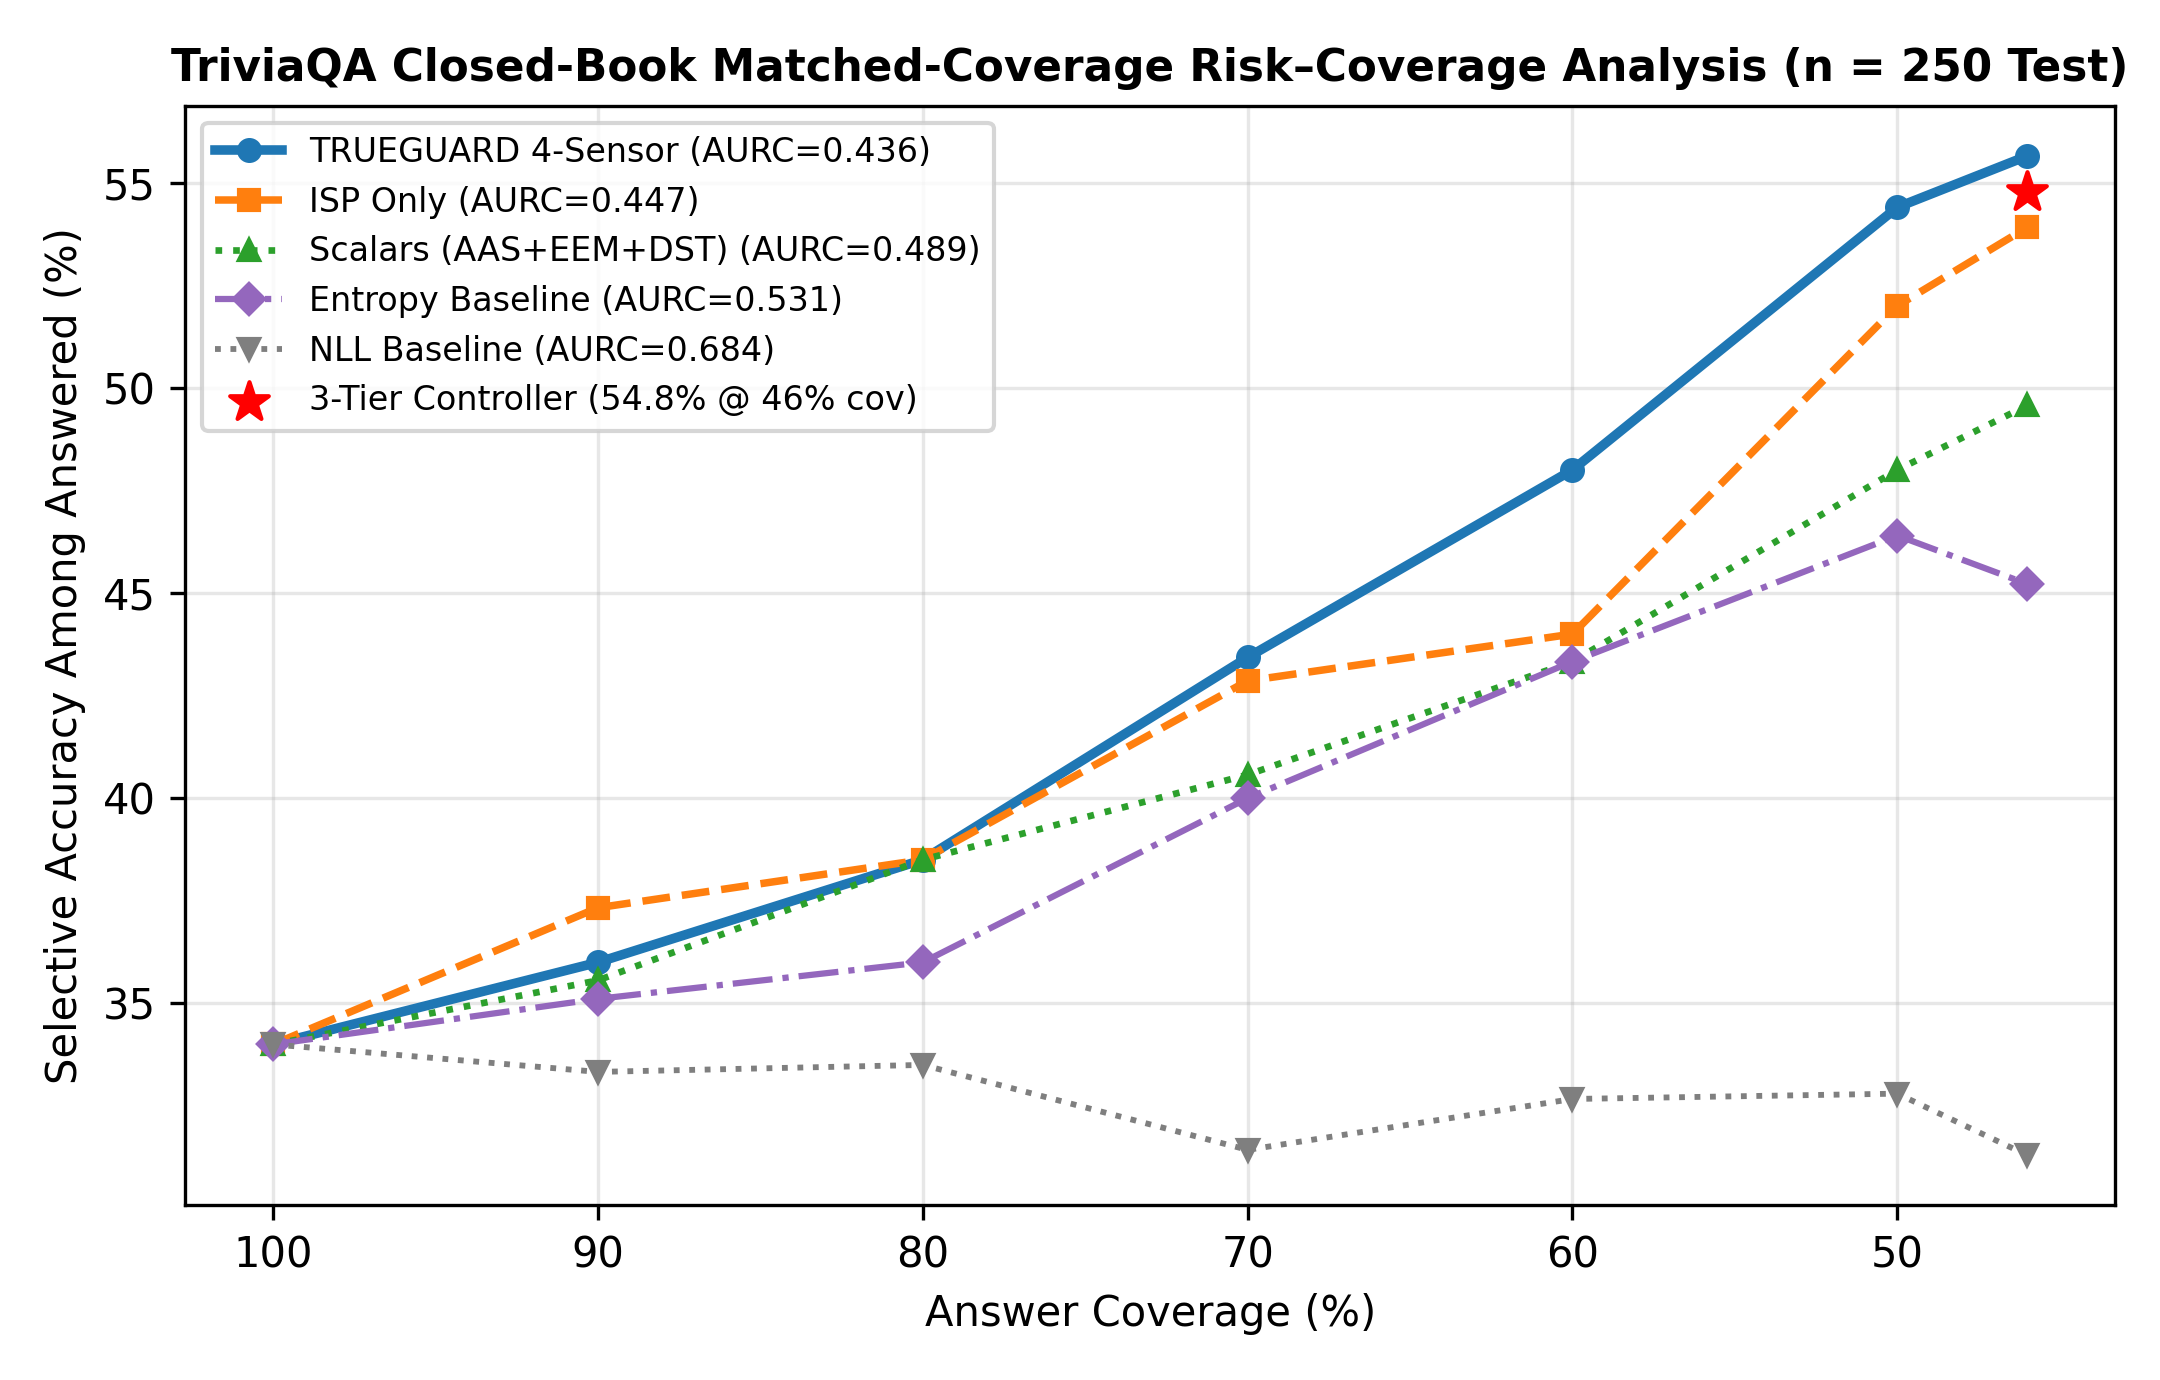
\includegraphics[width=\columnwidth]{figures/Fig3_TriviaQA_Matched_Coverage_RiskCurve.png}
\caption{Matched-coverage selective prediction accuracy across coverage thresholds on TriviaQA, comparing TRUEGUARD 4-sensor fusion with ISP-only, scalars-only, predictive entropy, length-normalized NLL, and the full 3-tier controller operating point (54.8\% at 46\% coverage).}
\label{fig:triviaqa_abstain}
\end{figure}

\subsection{Computational Efficiency}
\label{sec:res_efficiency}
To quantify single-pass monitoring overhead, we profiled sequential single-query decoding on a CUDA T4 GPU across 25 prompts and 24 forced tokens (\texttt{attn\_implementation="eager"}, \texttt{batch\_size = 1}; Table~\ref{tab:latency}). Vanilla TinyLlama averages 29.78~ms/token. TRUEGUARD post-pass monitoring averages 34.52~ms/token (+4.74~ms/token, +15.9\% overhead), which is 4.60 times faster than sequential 5-sample decoding (158.77~ms/token). Online per-token monitoring averages 37.84~ms/token (+8.06~ms/token, +27.1\% overhead), or 4.20 times faster than sequential 5-sample decoding.

These timings are not directly comparable to the external baseline Colab run, where $M = 10$ samples were generated in parallel (\texttt{batch\_size = 10}) using PyTorch's \texttt{sdpa} attention kernel with early end-of-sequence stopping (0.6545~s/query for sampling plus 0.0523~s/query for SelfCheckGPT NLI, omitting the initial greedy pass, totaling 0.7068~s/query; Semantic Entropy totaled 1.6622~s/query including 1.0078~s/query for bidirectional DeBERTa-large NLI and 2.47~GB peak NLI VRAM). Because the attention kernels, batch sizes, and sequence-length controls differed, our timing experiments do not establish an end-to-end wall-clock speed advantage over optimized batched SelfCheckGPT-NLI. TRUEGUARD's verified efficiency advantages are architectural (one LLM generation and zero external 435M-parameter NLI models) and sequential (4.20 to 4.60 times lower latency under matched sequential single-query serving).

\begin{table}[t]
\centering
\caption{Controlled Sequential Inference Latency Profiling on CUDA T4 (\texttt{eager}, \texttt{bs=1}, $25 \times 24$ Tokens)}
\label{tab:latency}
\resizebox{\columnwidth}{!}{%
\begin{tabular}{lccc}
\toprule
Decoding Configuration & Latency (ms/tok) & Overhead & vs.\ 5$\times$ Seq. \\
\midrule
Vanilla TinyLlama-1.1B (Greedy) & 29.78 & N/A & 5.33$\times$ \\
TRUEGUARD Post-Pass Monitoring & 34.52 & +4.74 (+15.9\%) & \textbf{4.60$\times$} \\
TRUEGUARD Online Monitoring & 37.84 & +8.06 (+27.1\%) & \textbf{4.20$\times$} \\
Sequential 5$\times$ Multi-Sample & 158.77 & +129.00 (+433.2\%) & 1.00$\times$ \\
\bottomrule
\end{tabular}}
\end{table}

% ==============================================================================
\section{Discussion}
\label{sec:discussion}

\subsection{Interpretation of the Main Findings}
The experimental evidence indicates that single-pass white-box hallucination detection on a frozen small language model is neither uniformly reliable nor merely an artifact of benchmark construction. Instead, detection performance depends strongly on three interacting conditions: the presence of surface artifacts in the evaluation benchmark, the availability of target-domain supervision, and whether risk estimates are used for abstention or active repair. Within a fixed domain, linear hidden-state probes capture error-related signals beyond answer length and surface n-grams. Across domains, however, those linear boundaries fail without target-domain refitting, and multi-sensor fusion offers little advantage over ISP alone once target probes are trained.

\subsection{Effect of Benchmark Artifacts}
Our artifact controls illustrate why reporting raw in-domain AUROC on synthetic benchmarks can mislead readers. On HaluEval-QA, answer length alone reaches 0.9572 AUROC; on HaluEval-Summarization, answer-text TF-IDF alone reaches 0.9539. Without controlling for these cues, a detector's 0.9880 or 0.9936 AUROC could easily be mistaken for deep factual understanding. Even though TRUEGUARD retains statistically significant gains over TF-IDF under strict length matching, residual lexical or structural regularities may still exist in paired teacher-forced benchmarks. Future white-box evaluations should therefore report length-matched and text-only TF-IDF baselines alongside neural metrics by default.

\subsection{Domain Shift and Detector Reliability}
The sharp gap between within-domain split-half probe alignment (+0.1125 to +0.6707 at $N = 900$) and cross-domain alignment (-0.0151 to +0.0204) is consistent with domain-dependent linear decision boundaries inside the frozen representation space. That domain dependence explains both why zero-shot pooled transfer collapses to chance (0.4597 to 0.5205 on Datasets 6 through 9, and 0.5504 on TriviaQA) and why simple probability recalibration (SrcRecal) cannot recover accuracy. Because pooled fusion also assigns over 96\% of its standardized weight to ISP, it suppresses auxiliary uncertainty signals even on natural benchmarks such as FaithDial and XSum where $\text{EEM}_{\text{mean}}$ carries genuine length-free discrimination.

\subsection{Value and Limitations of Few-Shot Refitting}
Target-domain few-shot refitting (training fresh probes from scratch on $K$ target examples in under 2~s on CPU) clarifies both the promise and the boundaries of lightweight supervision. When only 50 target labels are available, fitting 2,048-dimensional linear probes overfits relative to 1D EEM or TF-IDF. At 250 target labels, refitted white-box probes deliver clear gains on FaithDial, FEVER, and WikiBio-GPT3 while cutting ECE sharply, yet merely tie 1D answer length on XSum-Factuality. Supervision also changes how external baseline comparisons must be read: on TriviaQA, TRUEGUARD's competitive performance against 10-sample SelfCheckGPT-NLI and significant gain over 10-sample Semantic Entropy depend directly on those 250 labeled TriviaQA calibration examples, whereas both external baselines rank risk without target labels.

\subsection{Selective Abstention Versus Active Correction}
On closed-book TriviaQA, TinyLlama-1.1B answers only 34.00\% of questions correctly under greedy decoding. In that low-knowledge setting, risk-based selective abstention cleanly trades coverage for reliability, raising accuracy on answered questions to 55.65\% (64/115) and cutting system-wide errors to 20.40\%. Active Tier 1 stochastic resampling and Tier 2 single-passage Wikipedia retrieval repaired four errors but introduced three regressions on previously correct answers, yielding 54.78\% (63/115). On a 1.1B model with limited parametric recall and no high-precision external verifier, active self-repair cannot be assumed to improve upon pure selective abstention.

\subsection{Practical Implications}
For resource-constrained deployments running a frozen small LLM, these findings point to cautious engineering choices. When zero target labels exist, supervised white-box probes trained on external benchmarks should not be deployed zero-shot; single-pass 1D EEM or label-free multi-sample SelfCheckGPT-NLI are more dependable starting points. When roughly 250 labeled target examples can be collected, target-only ISP or TRUEGUARD refitting provides single-pass risk scoring without hosting an auxiliary NLI model, though practitioners should verify that it beats 1D length, 1D EEM, and TF-IDF on their specific task. Finally, calibrated risk scores should be paired with pure selective abstention unless an active retrieval or regeneration layer is explicitly validated to outperform abstention at matched coverage.

\subsection{Limitations and Threats to Validity}
Several limitations constrain how broadly these results can be generalized. First, every experiment uses one frozen 1.1B-parameter model (TinyLlama-1.1B-Chat-v1.0); larger 7B to 70B models possess richer parametric knowledge and may behave differently under domain shift or active retrieval. Second, Datasets 1 through 9 evaluate benchmark-provided responses through teacher forcing rather than free-form TinyLlama generations, and other unmeasured dataset artifacts beyond length and TF-IDF may remain. Third, the TriviaQA test set contains 250 questions, giving limited statistical power to separate TRUEGUARD (0.7876) from SelfCheckGPT-NLI (0.7477, $p_{\text{Holm}} = 0.478$) or ISP-only (0.7706, $p_{\text{Holm}} = 0.478$). Fourth, TRUEGUARD used 250 target-domain calibration labels on TriviaQA while SelfCheckGPT-NLI and Semantic Entropy were label-free for ranking. Fifth, Datasets 6 through 9 were inspected during zero-shot diagnosis before designing target-only refitting. Sixth, unsupervised white-box methods such as CCS \cite{burns2023discovering} and EigenScore/INSIDE \cite{chen2024inside} were not reproduced on TinyLlama-1.1B. Finally, controlled sequential latency timings do not establish a wall-clock speedup over GPU-batched \texttt{sdpa} SelfCheckGPT-NLI.

% ==============================================================================
\section{Conclusion and Future Work}
\label{sec:conclusion}

\subsection{Conclusion}
This study examined whether single-pass white-box signals extracted from a frozen small language model (TinyLlama-1.1B-Chat-v1.0) can reliably detect hallucinations across in-domain benchmarks, domain shift, and closed-book selective prediction. Across ten datasets and 32,590 evaluated sequences, our experiments support three balanced conclusions. First, raw in-domain AUROCs on synthetic benchmarks such as HaluEval-QA (0.9880) and HaluEval-Summarization (0.9936) are strongly inflated by answer-length and surface-text artifacts, yet TRUEGUARD still significantly beats answer-text TF-IDF under strict length matching (0.7901 to 0.9939 AUROC, $p \le 0.035$), with ISP carrying over 96\% of the fusion weight. Second, zero-shot pooled probes collapse to chance across four unseen domains (0.4597 to 0.5205) and on TriviaQA (0.5504), consistent with domain-dependent linear decision boundaries observed under equal-sample-size cosine controls. Target-domain few-shot refitting from scratch ($K = 250$) yields task-dependent gains on FaithDial, FEVER, and WikiBio-GPT3, whereas simpler baselines match or outperform TRUEGUARD at $K = 50$ and on XSum-Factuality. Third, on closed-book TriviaQA, target-refitted single-pass TRUEGUARD ($K = 250$, 0.7876 AUROC, 0.4360 AURC) significantly outperforms label-free Semantic Entropy, Predictive Entropy, and verified length-normalized NLL, and performs competitively with label-free SelfCheckGPT-NLI without external NLI models, while forensic auditing shows that selective abstention (55.65\%) rather than active Tier 1 or Tier 2 intervention (54.78\%) drives error reduction.

\subsection{Future Work}
Because these findings are bounded by a single 1.1B frozen model and a 250-question closed-book test split, future research should replicate this artifact-controlled and supervision-aware evaluation across larger open-weight LLMs (7B to 70B) and larger generation test sets ($n \ge 1{,}000$). Further work should also investigate genuine cross-domain transfer methods, such as low-rank probe adaptation or unsupervised representation alignment, that can outperform target-only refitting at $K \le 50$, compare against reproduced unsupervised white-box baselines (CCS and EigenScore), and test whether stronger dense retrieval pipelines enable active factual correction to surpass pure selective abstention.

% ==============================================================================
\bibliographystyle{IEEEtran}
\bibliography{references}

\begin{IEEEbiographynophoto}{Yogesh Ravi M}
is with the School of Computer Science and Engineering, Vellore Institute of Technology, Chennai, Tamil Nadu, India. His research interests include large language models, hallucination detection, internal model representations, and trustworthy artificial intelligence.
\end{IEEEbiographynophoto}

\begin{IEEEbiographynophoto}{T. S. Pradeep Kumar}
(Senior Member, IEEE) is a Professor with the School of Computer Science and Engineering, Vellore Institute of Technology, Chennai, Tamil Nadu, India. He is a Senior Member of IEEE and a Senior Member of ACM. His research interests include artificial intelligence, machine learning, and trustworthy computing systems.
\end{IEEEbiographynophoto}

\EOD

\end{document}
